% File: diploma.tex

\documentclass[
    14pt,
    specialist,
    candidate, % document type
    subf, % use and configure subfig package for nested figure numbering
    href,
    dotsinheaders=false
]{disser}

\hypersetup{colorlinks=false} % Configure hyperref loaded by disser class

% Кодировка и язык
\usepackage[T2A]{fontenc} % поддержка кириллицы
\usepackage[utf8]{inputenc} % кодировка исходного текста
\usepackage[english,russian]{babel} % переключение языков

% Геометрия страницы и графика
\usepackage[a4paper, mag=1000, left=3cm, right=1.5cm, top=2cm, bottom=2cm, headsep=0.7cm, footskip=1cm]{geometry}
\usepackage{graphicx} % подключение графики
\usepackage{pdfpages} % вставка pdf-страниц

% Таблицы
\usepackage{array} % расширенные возможности для работы с таблицами
\usepackage{tabularx} % автоматический подбор ширины столбцов
\usepackage{dcolumn} % выравнивание чисел по разделителю

% Математика
\usepackage{bm} % полужирное начертание для математических символов
\usepackage{amsmath} % дополнительные математические возможности
\usepackage{amssymb} % дополнительные математические символы
\usepackage{times}

% Библиография и ссылки
\usepackage{cite} % поддержка цитирования
% \usepackage[colorlinks=false]{hyperref} % Removed - loaded by 'href' class option
% \urlstyle{same}
% \renewcommand{\UrlFont}{\rmdefault}

% Прочее
\usepackage{color} % работа с цветом
\usepackage{epstopdf} % конвертация eps в pdf
\usepackage{multirow} % объединение ячеек таблиц по вертикали
\usepackage{afterpage} % вставка материала после текущей страницы
\usepackage{indentfirst} % отступ в первом абзаце раздела
\usepackage[font={normal}]{caption} % настройка подписей к рисункам и таблицам
\usepackage[onehalfspacing]{setspace} % полуторный интервал
\usepackage{fancyhdr} % установка колонтитулов
\usepackage{paratype} % моноширинный кириллический шрифт
\usepackage{listings} % поддержка вставки исходного кода
% \usepackage{newtxtext}
% \usepackage{newtxmath}
\usepackage{enumitem} % для настройки списков

% % Установка шрифта Times New Roman
\renewcommand{\rmdefault}{ftm}

% Установка абзацного отступа 1.25 см
\setlength{\parindent}{1.25cm}

% Убрать дополнительный интервал между абзацами одного стиля
\setlength{\parskip}{0pt}

% Настройка списков
\setlist{nosep} % убираем дополнительные отступы в списках
\setlist[itemize,1]{label={\textbullet}} % первый уровень маркированного списка
\setlist[itemize,2]{label={\textendash}} % второй уровень маркированного списка
\setlist[enumerate,2]{label={\alph{)}.}} % второй уровень нумерованного списка
\setlist[enumerate,1]{label={\arabic*.}, leftmargin=1.25cm, labelwidth=1cm, labelsep=0.25cm}

% Настройка стиля страницы
\pagestyle{fancy}      % Использование стиля "fancy" для оформления страниц
\fancyhf{}              % Очистка текущих значений колонтитулов
\fancyfoot[C]{\thepage} % Установка номера страницы в нижнем колонтитуле по центру
\renewcommand{\headrulewidth}{0pt} % Удаление разделительной линии в верхнем колонтитуле


% Настройка подписей к таблицам и рисункам
\captionsetup[table]{position=above, justification=raggedright, singlelinecheck=false, format=plain, labelformat=simple, labelsep=endash}
\captionsetup[figure]{position=below, justification=centering, singlelinecheck=true, format=plain, labelformat=simple, labelsep=endash}

% Настройка шрифта в таблицах
\let\oldtabular\tabular
\let\endoldtabular\endtabular
\renewenvironment{tabular}{\small\oldtabular}{\endoldtabular}

\makeatletter

% Define tab command for consistent spacing
\newcommand\tab[1][1.25cm]{\hspace*{#1}}

% Fix TOC to include dots between titles and page numbers
\renewcommand\@dotsep{4.5}
\renewcommand\tocpostthepart{\@postskip}
\renewcommand\tocpostthechapter{\@postskip}
\renewcommand\tocpostthesection{\@postskip}
\renewcommand\tocpostthesubsection{\@postskip}
\renewcommand\tocpostthesubsubsection{\@postskip}
\renewcommand\tocposttheparagraph{\@postskip}
\renewcommand\tocpostthesubparagraph{\@postskip}
% \renewcommand{\UrlFont}{\normalfont}

% Redefine TOC entry commands to use 14pt font and include dots
\renewcommand*\l@chapter[2]{%
  \ifnum \c@tocdepth >\m@ne
    % \vskip 1.0em \@plus\p@
    \setlength\@tempdima{2em}%
    \begingroup
    \parindent \z@ \rightskip \@pnumwidth
    \parfillskip -\@pnumwidth
    % \leavevmode \normalsize\bfseries\fontsize{14}{16}\selectfont
    \hskip -\leftskip
    #1\nobreak\leaders\hbox{\normalfont$\m@th\mkern \@dotsep mu\hbox{.}\mkern \@dotsep mu$}\hfill\nobreak\hb@xt@\@pnumwidth{\hss #2}\par
    \penalty\@highpenalty
    \endgroup
  \fi}

\renewcommand*\l@section[2]{%
  \ifnum \c@tocdepth >\z@
    % \vskip 1em \@plus\p@
    \setlength\@tempdima{2em}%
    \begingroup
    \parindent \z@ \rightskip \@pnumwidth
    \parfillskip -\@pnumwidth
    % \leavevmode \normalsize\fontsize{14}{16}\selectfont
    \hskip -\leftskip
    #1\nobreak\leaders\hbox{\normalfont$\m@th\mkern \@dotsep mu\hbox{.}\mkern \@dotsep mu$}\hfill\nobreak\hb@xt@\@pnumwidth{\hss #2}\par
    \penalty\@highpenalty
    \endgroup
  \fi}

\renewcommand*\l@subsection[2]{%
  \ifnum \c@tocdepth >\@ne
    % \vskip 1em \@plus\p@
    \setlength\@tempdima{3em}%
    \begingroup
    \parindent \z@ \rightskip \@pnumwidth
    \parfillskip -\@pnumwidth
    \leavevmode \normalsize\fontsize{14}{16}\selectfont
    \hskip -\leftskip
    #1\nobreak\leaders\hbox{\normalfont$\m@th\mkern \@dotsep mu\hbox{.}\mkern \@dotsep mu$}\hfill\nobreak\hb@xt@\@pnumwidth{\hss #2}\par
    \penalty\@highpenalty
    \endgroup
  \fi}

% Add a flag to track if we're immediately after a chapter
\newif\if@afterchapter
\@afterchapterfalse

% Make chapter titles bold and centered with proper anchoring - ALL CAPS for first level
\newcommand{\mychapter}[1]{%
  \newpage
  \refstepcounter{chapter}% Move counter increment inside the command
  \hypertarget{chap:\thechapter}{}% Create unique anchor
  \begin{center}
    \textbf{\MakeUppercase{\thechapter\space #1}}
  \end{center}
  % Reduce space between number and title in TOC by using less space or negative space
  \addcontentsline{toc}{chapter}{\texorpdfstring{\thechapter\hspace{0.3em}#1}{Chapter \thechapter}}% Reduced space
  \@afterchaptertrue % Set flag after chapter
}

% Special command for unnumbered chapters (like INTRODUCTION, CONCLUSION)
\newcommand{\myunnumberedchapter}[1]{%
  \newpage
  \hypertarget{chap:#1}{}% Create unique anchor
  \begin{center}
    \textbf{\MakeUppercase{#1}}
  \end{center}
  \addcontentsline{toc}{chapter}{\texorpdfstring{#1}{#1}}% Add optional PDF string
}

\newcommand{\mysection}[1]{%
  \ifnum\value{section}>0
  \vspace{1em}
  \fi
  \refstepcounter{section}
  \hypertarget{sec:\thechapter.\thesection}{}% Create unique anchor
  \textbf{\thesection\space #1}
  % Reduce space between number and title in TOC
  \addcontentsline{toc}{section}{\texorpdfstring{\thesection\hspace{2em}#1}{Section \thesection}}% Reduced space
}

\newcommand{\mysubsection}[1]{%
  \refstepcounter{subsection}
  \hypertarget{subsec:\thechapter.\thesection.\thesubsection}{}
  \textbf{\thesubsection\space #1}
  % Reduce space between number and title in TOC
  \addcontentsline{toc}{subsection}{\texorpdfstring{\thesubsection\hspace{2em}#1}{Subsection \thesubsection}}
}

\renewcommand{\thechapter}{\arabic{chapter}}

% Define appendix format with Cyrillic letters
\newcommand{\startappendix}{%
  \setcounter{chapter}{0}%
  \renewcommand{\thechapter}{\CYRA\cyrillictext}%
  \renewcommand{\thesection}{\thechapter.\arabic{section}}%
  \renewcommand{\thesubsection}{\thechapter.\arabic{section}.\arabic{subsection}}%
  \renewcommand{\thetable}{\thechapter.\arabic{table}}%
  \renewcommand{\thefigure}{\thechapter.\arabic{figure}}%
}

\makeatother

\AtBeginDocument{\onehalfspacing}

% Настройка листингов кода (перед \begin{document})
\lstset{
    basicstyle=\normalsize\ttfamily,        % базовый шрифт нормального размера
    numberstyle=\normalsize\ttfamily,       % шрифт нумерации того же размера
    numbers=left,                           % нумерация строк слева
    numbersep=6pt,                          % отступ номеров от кода
    frame=single,                           % единая рамка
    framerule=0.8pt,                        % толщина рамки
    framexleftmargin=17pt,                  % рамка захватывает номера строк
    xleftmargin=17pt,                       % отступ слева для выравнивания
    captionpos=t,                           % заголовок сверху
    breaklines=true,                        % перенос длинных строк
    showstringspaces=false,                 % не показывать пробелы в строках
    resetmargins=true,                      % сброс полей
    aboveskip=10pt,                         % отступ сверху
    belowskip=10pt                          % отступ снизу
}

% Переопределение названий для листингов
\renewcommand{\lstlistingname}{Листинг}

% Настройка подписей к листингам через caption
\captionsetup[lstlisting]{
    singlelinecheck=false,
    justification=raggedright,
    format=plain,
    labelformat=simple,
    labelsep=endash
}

% Настройка формата номеров листингов
\makeatletter
\AtBeginDocument{
  % Переопределение формата номера листинга
  \renewcommand{\thelstlisting}{\arabic{lstlisting}}
}
\makeatother

\begin{document}

\sloppy


\includepdf[pages={1-5}]{./assets/TitlePage.pdf}

\renewcommand{\contentsname}{\centerline{\normalsize\bfseries\centerline{\textbf{\MakeUppercase{СОДЕРЖАНИЕ}}}}}
\setcounter{tocdepth}{1}

\tableofcontents

\myunnumberedchapter{ВВЕДЕНИЕ}

В современной инновационной экономике проблема эффективного распределения ресурсов на ранних стадиях развития проектов остается одной из наиболее остро стоящих. Существующие механизмы финансирования, от традиционного венчурного капитала до акселерационных программ, зачастую не способны ответить на вызовы с которыми сталкиваются начинающие проекты. Неравномерное распределение информации, субъективизм в оценках, ошибки на этапе проверки гипотез. Это порождает значительные барьеры, особенно для тех, кто стремится быстро и с минимальными издержками валидировать идеи, не попадая в зависимость от длительных циклов отбора или ограниченных грантовых программ.

На этом фоне возникает объективная потребность в создании альтернативной системы, обеспечивающей более прозрачную, масштабируемую модель распределения инвестиционных ресурсов. В настоящей работе рассматривается подход к построению такой системы на основе блокчейн-технологий и алгоритмов коллективной оценки, способной выполнять функции рыночной валидации идей. Предлагаемый механизм устраняет ряд фундаментальных ограничений традиционных моделей: снижает асимметрию информации, минимизирует субъективность принятия решений, создает непрерывный процесс валидации идеи, предотращает возможность манипуляций со стороны участников.

Актуальность исследования определяется необходимостью разработки эффективного и воспроизводимого способа взаимодействия между стартапами и инвесторами на начальных стадиях, способного ускорить трансформацию идей в реальные проекты.

Целью данной работы является реализация технологии для распределения инвестиций на основе коллективных оценок в кроссплатформенном приложении.

Для достижения поставленной цели в работе решаются следующие задачи:
\begin{enumerate}
  \item Проанализировать предметную область и целевую аудиторию.
  \item Сравнить существующие аналогичные решения.
  \item Проанализировать современные способы распределения ресурсов.
  \item Определить функциональные требования.
  \item Представить процесс распределения ресурсов в виде формальной схемы.
  \item Составить экономическое обоснование процесса распределения ресурсов для применения в предметной области.
  \item Перевести принцип работы системы в математическую и программную форму.
  \item Разработать пользовательские сценарии.
  \item Спроектировать архитектуру и структуру базы данных кроссплатформенного приложения.
  \item Разработать серверную часть кроссплатформенного приложения.
  \item Разработать клиентскую часть кроссплатформенного приложения.
  \item Проанализировать результаты и перспективы дальнейшего внедрения.
\end{enumerate}

Предметом исследования являются механизмы распределения ресурсов и оценки инновационных проектов на ранних стадиях, основанные на технологиях блокчейн и искусственного интеллекта. Объектом исследования выступает процесс инвестирования в ранние стадии инновационных проектов.

Практическая значимость работы заключается в создании новой парадигмы инвестирования, которая позволит преодолеть структурные ограничения существующих механизмов и обеспечить более эффективное распределение капитала для инновационных проектов.

% ## 1
\mychapter{АНАЛИТИЧЕСКИЙ ОБЗОР}

% ### 1.1
\mysection{Анализ предметной области}

Рынок инвестиций в стартапы на ранних стадиях представляет собой сложную и многогранную экосистему, в которой участвуют разнообразные субъекты – от основателей и индивидуальных инвесторов до венчурных фондов и корпоративных акселераторов. Такая экосистема характеризуется высокой степенью неопределенности и информационной асимметрией, что приводит к появлению структурных проблем, негативно влияющих на эффективность распределения ресурсов.

Это приводит к тому, что перспективные проекты с несовершенной маркетинговой стратегией или без связей остаются незамеченными. За счет узкого охвата потенциальных инвесторов субъективность оценки, основанная на личных впечатлениях или косвенных сигналах (например, репутации основателя) усиливает предвзятость.

Эта асимметрия порождает систематическую субъективность в оценках: решения о финансировании по большей части принимаются на основе неформализованных критериев и «интуитивных» сигналов, а не объективных метрик. Вследствие этого капитал концентрируется вокруг ограниченного круга проектов, которые получают повышенное внимание за счёт лучших контактов или более ярких презентаций, тогда как остальные идеи, не обладающие значительной социальной поддержкой, оказываются без шансов на развитие.

Кроме того, отсутствие встроенных механизмов ликвидности создаёт экономический разрыв между стадиями запуска и выхода из проекта: инвесторы вынуждены искать внешние площадки или договариваться о выкупе долей, что замедляет оборот капитала и увеличивает транзакционные издержки. Наконец, устойчивость инновационной экосистемы подрывает эффект «инвестиционных каскадов», когда решения небольшого круга лидирующих инвесторов задают тренд для всего рынка, нивелируя разнообразие взглядов и препятствуя объективной проверке гипотез.

Эти вызовы приводят к неоптимальному распределению капитала, замедляя развитие инновационной экосистемы. Именно в этой среде, где традиционные финансовые инструменты оказываются неприспособленными к особенностям распределённых сетей, появляется острая потребность в механизмах, способных объективно агрегировать коллективную экспертизу, автоматически устанавливать ценность проектов и обеспечивать устойчивую ликвидность.

Анализ текущей динамики венчурного рынка демонстрирует институционализацию стартапов как полноценного элемента современной экономики. Согласно данным Global Innovation Index 2024 \cite{gii2024}, доля венчурных инвестиций по отношению к ВВП уверенно растёт не только в странах с высоким уровнем дохода, но и в странах со средним уровнем развития, что показано на рисунке~\ref{fig:vc-gdp-share}. Это свидетельствует о снижении барьеров для вхождения в стартап-экосистему и подтверждает всё более системную роль стартапов в экономическом росте и распределении инновационного капитала.

\begin{figure}[h]
  \centering
  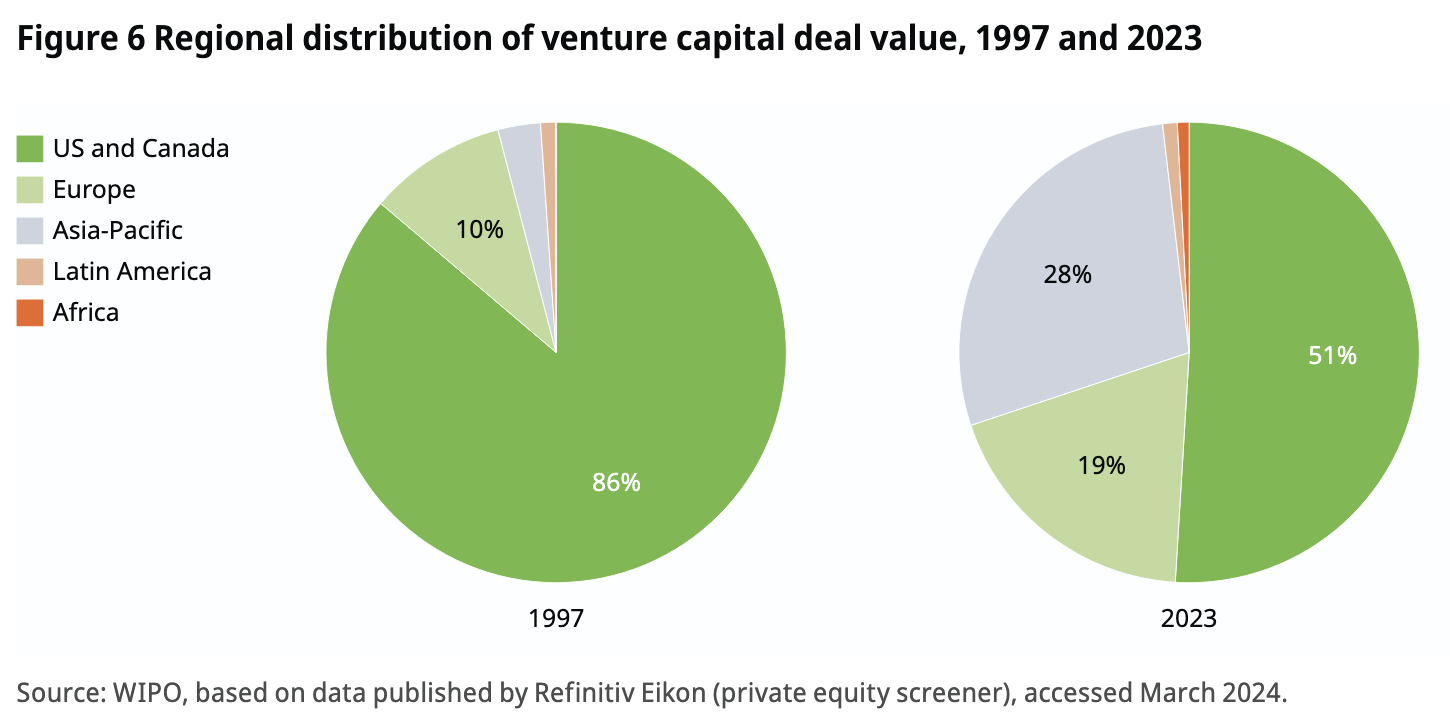
\includegraphics[width=0.75\textwidth]{assets/vc-gdp-share.png}
  \caption{Доля венчурных инвестиций по отношению к ВВП в странах с различным уровнем дохода. Источник: Global Innovation Index 2024~\cite{gii2024}.}
  \label{fig:vc-gdp-share}
\end{figure}

Анализ предметной области инвестиций в стартапы ранних стадий демонстрирует, что на этом этапе стоимость проектов формируется не реальными денежными потоками, а ожиданиями и верой участников экосистемы. Отсутствие стабильных финансовых показателей заставляет инвесторов полагаться на фрагментарные данные — результаты первых прототипов, отзывы пользователей, а порой и просто репутацию команды — что приводит к существенной информационной асимметрии.

% ### 1.2
\mysection{Определение актуальности}

Основатели стартапов сталкиваются с необходимостью быстрой проверки своих идей на жизнеспособность.Традиционные механизмы, такие как венчурный капитал или акселерационные программы, часто требуют длительных циклов отбора, раскрытия критически важной информации и подчинения строгим условиям, что создает барьеры для быстрой рыночной валидации. В то же время инвесторы, ориентированные на диверсификацию портфеля за счет перспективных, но еще не оформившихся инициатив, нуждаются в надежных инструментах для оценки широкого спектра проектов и оптимального распределения капитала. Текущие подходы, основанные на дискретных инвестиционных раундах, ограничивают выборку доступных стартапов и усиливают монополию крупных игроков, оставляя множество потенциально прорывных идей без поддержки.

Одной из ключевых проблем является информационная асимметрия между основателями стартапов и потенциальными инвесторами. Основатели обладают глубоким пониманием своих проектов, однако при необходимости привлечения инвестиций вынуждены подстраивать это понимание под маркетинговый контекст. В свою очередь, инвесторы ограничены в доступе к полной информации о проекте и его перспективах, что затрудняет объективную оценку и вынуждает опираться на косвенные сигналы, такие как образование и опыт основателей.

Особенно ярко это проявляется в блокчейн стартапах, ведь им необходим пул ликвидности для обеспечения бесперебойной торговли, стабильности цен и доверия пользователей к их токену или платформе. Пул ликвидности — это резерв цифровых активов, хранящийся в блокчейне и предназначенный для автоматического обмена токенов по заранее установленным правилам без участия посредников.

Обеспечение достаточного уровня ликвидности является фундаментальным условием эффективного функционирования блокчейн-стартапов, поскольку именно она обеспечивает непрерывность торговых операций, минимизирует проскальзывание и способствует поддержанию стабильности ценового уровня токена. Глубокая ликвидность выступает индикатором здоровой экосистемы, привлекает трейдеров, предпочитающих площадки с низкой ценовой волатильностью, и формирует доверие инвесторов к проекту, что, в свою очередь, усиливает сетевой эффект и стимулирует дальнейшее расширение пользовательской базы. При недостаточном объёме ликвидности даже незначительные сделки способны вызвать существенные колебания цены, создавая угрозу массового оттока участников и повышая риски ценовых манипуляций со стороны крупных держателей.

Достижение и поддержание необходимого уровня ликвидности осуществляется с помощью ряда финансовых и организационных подходов. В первую очередь, для быстрого привлечения средств используются программы, которые поощряют участников сообщества размещать свои активы в пулах за вознаграждение. Другим распространённым способом является первичное размещение токенов на децентрализованных биржах, позволяющее одновременно привлечь инвестиции и сформировать начальный резерв активов для торговли.

Также применяется подход, при котором сам проект выпускает специальные облигации или аналогичные финансовые инструменты, чтобы напрямую владеть ликвидностью, избегая зависимости от временных внешних вложений.

Ещё одним вариантом является привлечение профессиональных организаций, специализирующихся на создании ликвидности, что позволяет обеспечить необходимый объём активов для торговли без значительных собственных расходов проекта.

Дополнительно используется размещение токенов на крупных централизованных биржах при поддержке профессиональных участников рынка, что расширяет круг потенциальных инвесторов и повышает популярность проекта.

Наконец, важным методом выступает применение автоматизированных алгоритмов, которые обеспечивают непрерывное формирование цен и постоянный доступ участников к торговле, снижая при этом резкие колебания цены и увеличивая доверие пользователей к платформе.

Комплекс этих проблем создаёт существенные барьеры для эффективного функционирования рынка инвестиций в ранние стадии, приводя к неоптимальному распределению капитала, когда перспективные проекты остаются без необходимой поддержки, а проекты с меньшим потенциалом, но лучшей презентацией или более сильными социальными связями, получают непропорционально большие инвестиции, что в конечном итоге снижает эффективность инновационной экосистемы и замедляет технологический прогресс.

% ### 1.3
\mysection{Описание целевой аудитории}

Портрет целевой аудитории платформы включает в себя две ключевые группы: основателей стартапов и инвесторы, ориентированных на высокорисковые, но потенциально доходные вложения.

Первую группу составляют преимущественно молодые люди от 20 до 35 лет. Они нуждаются в доступе к капиталу, который должен основываться на объективной оценке потенциала идеи, а не на субъективных факторах, таких как опыт, образование или социальные связи, что подтверждается тем, Отсутствие качественной обратной связи представляет существенное препятствие для развития их проектов. Они стремятся минимизировать затраты времени и ресурсов на привлечение инвестиций, что особенно актуально, учитывая, что процесс привлечения посевного финансирования в среднем занимает от шести до девяти месяцев.

Вторую группу составляют инвесторы ранних стадий, для которых важным является обеспечение доступа к качественному потоку сделок с высоким потенциалом. Помимо этого, инвесторам необходимы объективные данные для оценки потенциала проектов в условиях ограниченного объёма информации; Наконец, инвесторы стремятся к диверсификации инвестиционного портфеля, предпочитая инвестировать в большое кол-во проектов, что позволяет распределить риски, несмотря на ограничения, связанные с оценкой большого количества проектов.

Учитывая, что обе группы действуют в условиях высокой неопределённости и переизбытка информации, внимание становится дефицитным ресурсом. Рынок инноваций и венчурного капитала всё чаще функционирует по законам экономики внимания, где первичную роль играет не только содержание, но и форма подачи. Визуально привлекательный, яркий, интуитивно понятный интерфейс становится не просто инструментом взаимодействия с продуктом, а критическим фактором захвата и удержания пользователя, особенно в условиях растущей конкуренции за внимание. Он способствует не только улучшению пользовательского опыта, но и формирует доверие к технологической и инновационной зрелости платформы.

Проведённый анализ целевой аудитории демонстрирует, что, несмотря на различия в потребностях, стейкхолдеры заинтересованы в создании более эффективной, объективной и прозрачной системы оценки и финансирования инновационных проектов на ранних стадиях. В этом контексте яркий, современный и эмоционально вовлекающий интерфейс представляет собой не эстетическую деталь, а стратегически важный инструмент, способствующий расширению аудитории, повышению вовлечённости пользователей и достижению маркетинговых целей на конкурентном рынке.

% ### 1.4
\mysection{Обзор существующих решений}

В современной экосистеме инвестирования применяются различные подходы, каждый из которых частично решает обозначенные проблемы, но не способен обеспечить

Основные практики привлечения инвестиций включают традиционное венчурное финансирование, участие в акселерационных программах, краудфандинг.

Венчурные фонды и инвесторы представляют собой наиболее распространённый механизм финансирования ранних стадий, основанный на личных встречах, презентациях и субъективной оценке потенциала проектов и команд. Преимущества данного подхода заключаются в наличии доступа к экспертной поддержке и менторству, возможности установления долгосрочных отношений между основателями и инвесторами, гибкости в структурировании сделок и условия инвестирования, а также наличии широкой сети контактов, которую инвесторы могут предоставить. Однако существенные ограничения этого механизма проявляются в высокой степени субъективности и предвзятости при оценке проектов, Согласно \cite{imbierowicz2024peer}, оценки стартапов на ранних стадиях часто опираются не на бизнес-фундамент, а на ориентиры из недавних сделок в смежных сегментах, что приводит к эффекту переоценки и рыночной нестабильности. Дополнительно, зависимость от социальных связей и репутации, а также необходимость полного раскрытия идеи, создающая риск для интеллектуальной собственности и географическая концентрация венчурных инвестиций, ограничивающая доступ к капиталу для основателей из других регионов, существенно снижают эффективность данного подхода.

Акселераторы и стартап-инкубаторы, такие как Y Combinator, Techstars, AngelList, предлагают структурированные программы поддержки стартапов, объединяющие менторство, образовательные компоненты и доступ к инвесторам. Структурированный процесс отбора и поддержки проектов создаёт чёткие рамки для развития, что особенно важно для неопытных основателей \cite{thiel2014zero}, а доступ к обширным сетям контактов и экспертизе ускоряет валидацию идей и выход на рынок. При этом частичная автоматизация инвестиционных процессов снижает транзакционные издержки, а стандартизация документации упрощает юридические аспекты финансирования. Главной проблемой здесь является высокая конкуренция за места в ведущих программах (например, Y Combinator принимает менее 1\% заявителей \cite{yc_acceptance_rate}) значительно снижает шансы на участие и отсеивает потенциально хорошие идеи. Также, географические ограничения продолжают оставаться барьером для основателей, расположенных вне основных инновационных хабов.

\begin{figure}[ht!]
  \centering
  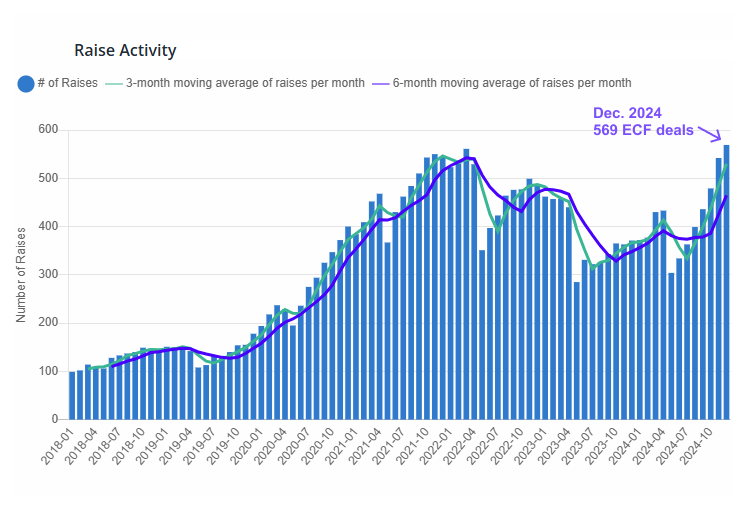
\includegraphics[width=0.8\textwidth]{./assets/crowd-funding.png}
  \caption{Рост числа инвестиций}
  \label{fig:regcf-investments}
  \label{fig:crowd-funding}
\end{figure}

Сравнительный анализ эффективности существующих подходов показывает, что ни один не способен обеспечить одновременно, объективную оценку проектов и оптимальное распределение капитала. Стоит отметить, что сильной стороной традиционных подходов является их структурированность и наличие экспертной поддержки, особенно в случае венчурных фондов и акселераторов, где стартапы получают доступ к опыту и связям \cite{lange2024angels}. Однако слабые стороны этих механизмов существенно ограничивают возможности их масштабирования.

% ### 1.5
\mysection{Требования к технической реализации}

Функциональные требования:
\begin{enumerate}
    \item Система должна предоставлять пользователю способ отправлять идею и делать её доступной для коллективной оценки.
    \item Пользователи должны иметь возможность выражать интерес к идее, влияя на её развитие и видимость.
    \item Идеи должны получать рыночную оценку.
    \item Администратор должен иметь возможность валидировать контент до его публикации на платформе.
    \item Система должна адаптироваться к изменению поведения участников для поддержания честности и эффективности.
\end{enumerate}

Нефункциональные требования:
\begin{enumerate}
    \item Совместимость: поддержка iOS, Android, Web и Telegram Mini Apps.
    \item Производительность: время отклика системы не должно превышать 30 секунд.
    \item Прозрачность: все финансовые операции и решения фиксируются в смарт-контрактах на публичном блокчейне.
    \item Модульность: архитектура должна быть компонентной с возможностью обновления, замены и масштабирования отдельных частей.
\end{enumerate}

% ### 1.6
\mysection{Вывод по первой главе}

Таким образом, проведенный анализ указывает на необходимость создания комплексного механизма, который бы одновременно обеспечивал объективную оценку проектов и оптимальное распределение капитала с учётом как объёма инвестиций, так и широты поддержки аудиторией.

% Глава 2
% ###############################################################
\mychapter{ТЕОРЕТИЧЕСКИЕ ОСНОВЫ РАСПРЕДЕЛЕНИЯ РЕСУРСОВ}

% ### 2.1 Обзор проблематики
\mysection{Предметная область}

Проблема распределения ресурсов охватывает широкий спектр дисциплин — от найма персонала и управления проектами до вычислительных систем, логистики и сетевой инфраструктуры. В формальном виде она сводится к оптимизации под ограничениями, где множество допустимых решений экспоненциально возрастает с ростом количества агентов, ресурсов и ограничений. При этом большинство задач относятся к классу NP-трудных, что делает невозможным их точное решение в разумное время и требует приближённых или эвристических подходов.

Даже в системах с чётко определёнными и конечными правилами, такими как шахматы, го или другие дискретные динамические среды, возникает экспоненциальный рост числа допустимых состояний. Например, в го количество возможных позиций оценивается порядка $10^{170}$, что значительно превышает любые физические пределы обработки. Аналогично, алгоритм AlphaZero \cite{silver2018general}, хотя и оперирует в рамках формализованных правил, демонстрирует, что оптимальное поведение в таких пространствах возможно лишь при использовании стохастических методов и обучения с подкреплением, поскольку алгоритмический перебор стратегий неосуществим.

Таким образом, несмотря на конечность правил и чёткую формализацию условий, многие реальные системы распределения ресурсов становятся неалгоритмизируемыми в силу экспоненциальной сложности и стратегической природы агентов. Это обосновывает необходимость перехода к децентрализованным, эмпирическим и конкурентным механизмам, которые перераспределяют вычислительную нагрузку, используют локальную информацию и допускают адаптивное поведение участников.

% ## 2.2
\mysection{Экономические принципы}

Рыночные механизмы — одна из самых ранних систем распределения, возникших естественным образом из человеческой потребности в обмене ресурсами.

Рынки представляют собой уникальный пример высокоэффективной распределённой системы, сформированной не посредством централизованного планирования, а в результате спонтанной самоорганизации. Исторически развитие рынков сопровождалось появлением новых форм коммуникации — от устных соглашений и письменных контрактов до телеграфа и цифровых платформ. Эти инновации способствовали расширению информационной пропускной способности рынков и увеличению точности передаваемых сигналов. В процессе обмена участники взаимодействуют в общих физических или цифровых пространствах — от рыночных площадей до онлайн-бирж — в результате чего формируется ключевой институциональный механизм: рыночная цена. Изначально сделки совершаются по индивидуально согласованным условиям, но с ростом числа участников рынок агрегирует информацию, и цены стремятся к единственному значению, отражающему консенсус оценок (рис.~\ref{fig:one-price}). Такая цена становится выражением коллективного знания, интегрируя разрозненные субъективные взгляды в объективный показатель.

\begin{figure}[h]
  \centering
  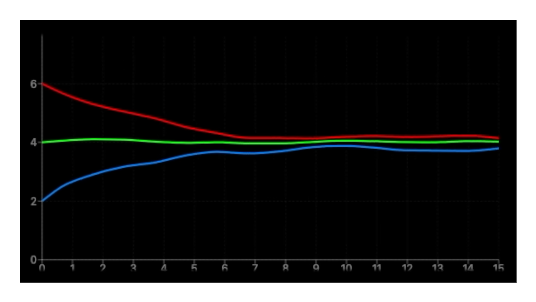
\includegraphics[width=0.9\textwidth]{./assets/one-price.png}
  \caption{Сходимость ценовых ожиданий участников рынка}
  \label{fig:one-price}
\end{figure}

Ещё одним важным аспектом является то, что вопреки ожиданиям, доступ к конфиденциальной информации не искажает рыночный сигнал. Наоборот, с точки зрения экономической теории, такие действия способствуют увеличению точности ценовых индикаторов. Участник, обладающий частной информацией, скрытыми знаниями или уникальной экспертизой стремится извлечь из неё выгоду, тем самым внося её в общедоступную цену, что в конечном итоге усиливает достоверность рыночных прогнозов.

Это свойство можно легко заметить, если сравнить графики глубины рынка для торговых пар с высокой и низкой ликвидностью (рис.~\ref{fig:limit-order}). Выраженная симметрия и плотность книги заявок в низколиквидных торговых парах свидетельствуют о высокой степени уверенности и согласованности ожиданий рыночных участников.

\begin{figure}[h]
  \centering
  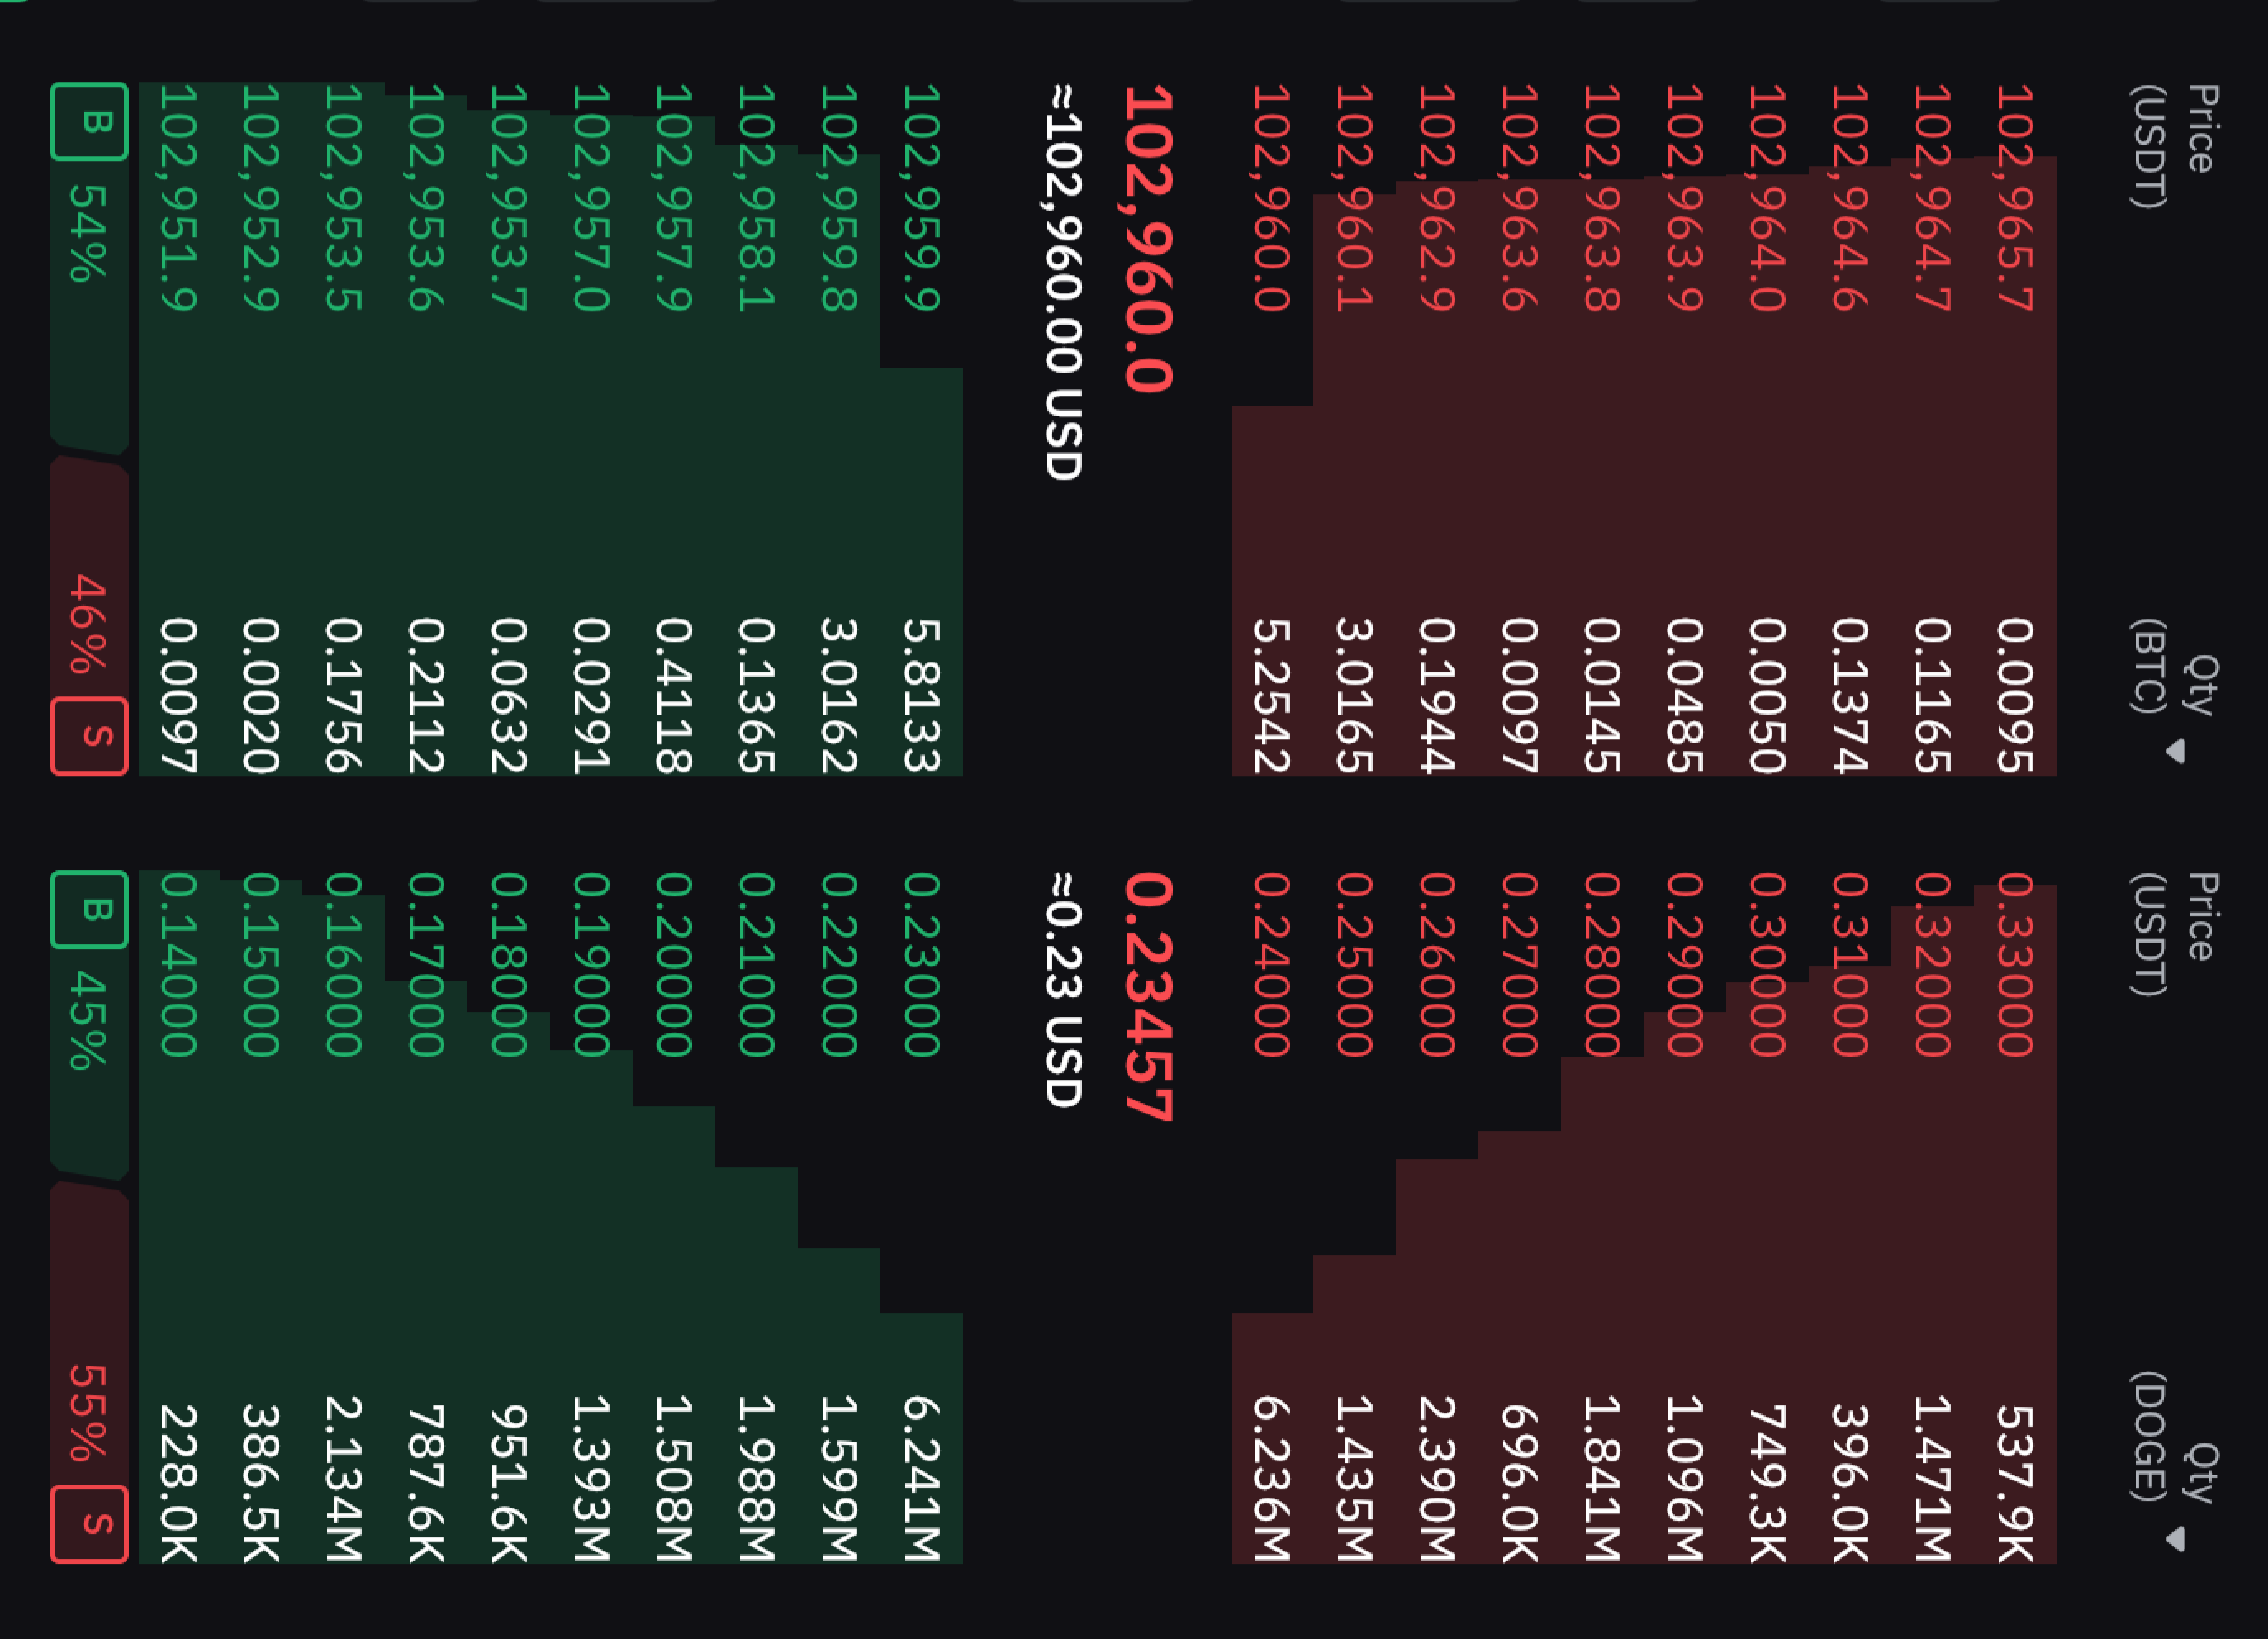
\includegraphics[width=0.9\textwidth]{./assets/limit-order.png}
  \caption{График глубины рынка для торговых пар с высокой и низкой ликвидностью}
  \label{fig:limit-order}
\end{figure}

Таким образом, рыночные цены становятся не просто индикатором текущего состояния, но и носителем предсказательной информации о будущем.

В этом контексте возникает важный вопрос: что произойдет, если мы отбросим настоящий компонент ценообразования и будем основывать торги только на будущих событиях. Отражение будущих ожиданий в ценах особенно ярко проявляется в таких примерах, как изменение стоимости фьючерсов на сельскохозяйственную продукцию в ответ на погодные прогнозы или изменение коэффициентов в букмекерских системах до фактического события \cite{wolfers2019price}. Одним из современных применений предсказательных рынков является проект Polymarket, использующий блокчейн для создания прозрачных и децентрализованных платформ прогнозирования.Самый известный прогноз Polymarket на сегодняшний день - президентские выборы в США в 2024 году за несколько недель до того, как стал известен результат. В результате системы такого рода обеспечивают высокий уровень точности предсказаний.

\begin{figure}[h]
  \centering
  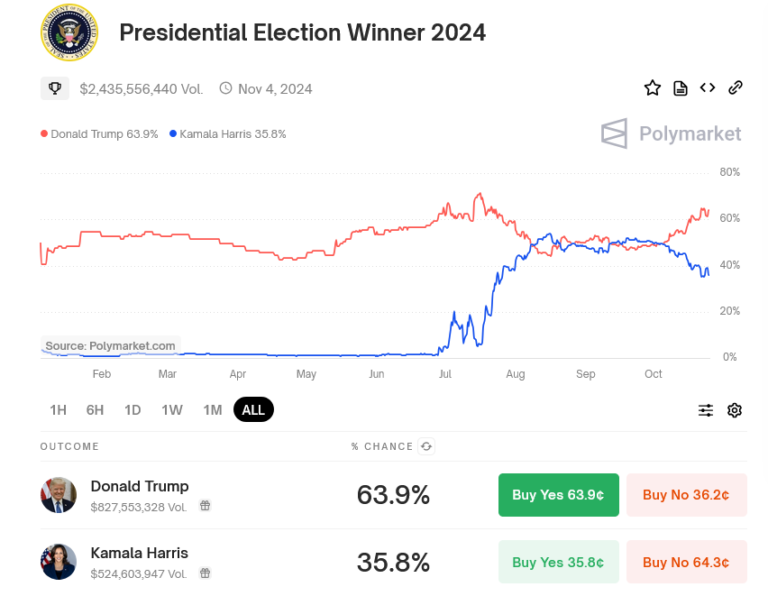
\includegraphics[width=0.9\textwidth]{./assets/polymarket-elections.png}
  \caption{Прогноз президентских выборов в США в 2024 году}
  \label{fig:polymarket-elections}
\end{figure}

Данные результаты демонстрируют возможность использования рыночных механизмов для предсказания будущих событий, а объединение традиционных рыночных механизмов с системами аналитики и вычислительными платформами формирует новую парадигму коллективного интеллекта \cite{berg2020prediction}.

Попробуем разобрать составные части подобных систем, чтобы получить представление о системе распределения ресурсов \ref{fig:bpmn-new}.

\begin{figure}[h]
  \centering
  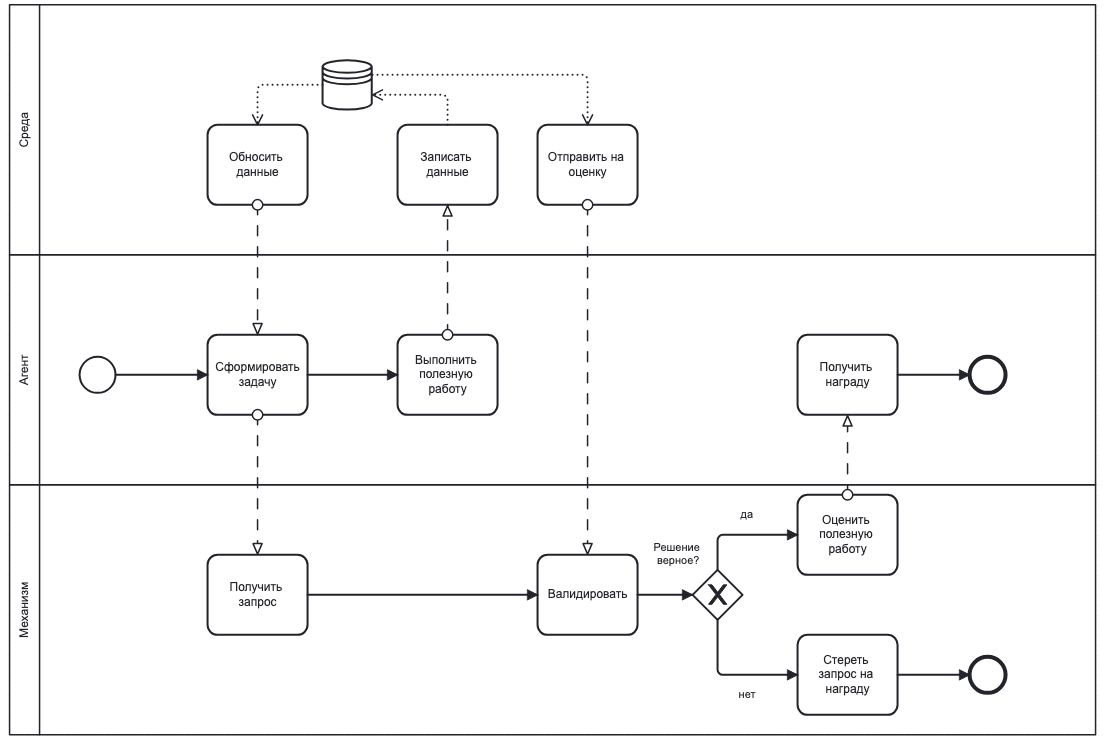
\includegraphics[width=0.8\textwidth]{./assets/bpmn-new.png}
  \caption{Формальная схема процесса распределения ресурсов}
  \label{fig:bpmn-new}
\end{figure}

% ## 2.3
\mysection{Вычислительная мощность}

Другими необходимым условием для того, чтобы механизм работал является наличие у агентов локальных экспертиз и отсутствие баесов для при принятии решений;

Каждый агент выполняет полезную работу, формируя выходные данные.
Через механизм согласования эти действия агрегируются в глобальное состояние, по которому затем все агенты синхронизируют новую итерацию.

?????
Равновесие нэша


%% ## 2.4
\mysection{Рациональная стратегия}

Необходимо заинтересовать агентов в выполнении полезной работы, так как любые косвенные или иерархические системы уступают прямому большинству (дестилляции коллективного знания) — прямой мажоритарной системе — по вероятности принятия «правильного» решения при условии независимости голосов и компетентности участников (p>0.5). Это демонстрирует, что децентрализованный рынок (прямое большинство) доминирует над всеми промежуточными схемами.

Согласно «Сondorcet's jury theorem» \cite{condorcet1785essay}, если у каждого участника системы вероятность дать правильную оценку чуть выше 50\%, то объединённое мнение группы с экспоненциальной вероятностью стремится к истине по мере роста размера группы.

Если даже индивидуальный агент обладает ограниченной информацией и баесом, при условии что участники системы заинтересованны давать правильные предсказания, при отсутствии координированных искажений, агрегирует разнообразные частичные знания, формируя более точное представление о будущем событии.

\begin{figure}[h]
  \centering
  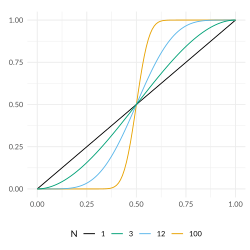
\includegraphics[width=0.7\textwidth]{./assets/condorcent.png}
  \caption{Вероятность для нескольких групп P преуспеть}
  \label{fig:condorcet}
\end{figure}

Следовательно, для эффективного функционирования механизма требуется трансформировать вероятностную модель, формируя такую экономическую среду, в которой соблюдение установленных правил становится единственной рациональной стратегией для участников.
Ключевым требованием является стимулирование агентов к выдаче максимально точных результатов. Если каждый агент обладает вероятностью $p > 0.5$ дать корректную оценку, то вероятность того, что большинство из $n$ участников примет правильное решение, вычисляется по формуле
\[
  \text{Pr}(\text{большинство правильно}) = \sum_{k=\lceil n/2 \rceil}^{n} \binom{n}{k} p^k (1-p)^{n-k},
\]

и при $p > 0.5$ стремится к единице по мере роста $n$. В иерархических или рекурсивных системах, где выход одних агентов служит входом для других, общая вероятность корректного результата по цепочке длины $k$ равна произведению
\[
  p_1 \times p_2 \times \cdots \times p_k,
\]

и остаётся выше $0.5$ для небольших $k$, если все $p_i > 0.5$. Более того, при наличии нескольких независимых путей вычисления итогового результата совокупная вероятность правильности определяется суммой соответствующих произведений, что дополнительно усиливает надёжность механизма.

% ## 2.5
\mysection{Система управления}

Если рассматривать все возможные задачи оптимизации или классификации (с одинаковой вероятностью), то любой алгоритм, который хорошо работает на одних задачах, неизбежно будет хуже на других. Иными словами, средняя производительность всех алгоритмов по всем возможным задачам одинакова.

Рассмотрим на примере хорошо известных механизмов решения подобных проблем. На одном пределе находится полностью централизованная система, в которой все решения принимает единый ИИ-агент. Такой подход обеспечивает простоту архитектуры и быструю реакцию на входные данные, а также возможность эффективно обрабатывать конфиденциальную информацию без её публичного раскрытия. Однако он нарушает принципы достоверной нейтральности: весовые коэффициенты модели содержат скрытые предпочтения, сама модель остаётся непрозрачной ввиду колоссальной сложности, а частые обновления (примерно каждые три месяца) создают дополнительную нагрузку на сопровождение и могут вносить непредсказуемые сдвиги в принятие решений.

Противоположный предел это Футархия \cite{Hanson2000}, которая опирается на рынки прогнозов, предполагая, что свободная торговля информацией порождает наилучшие коллективные решения, однако именно эта зависимость от торговли делает механизм уязвимым. Во-первых, ликвидность предсказательных контрактов редко бывает достаточной: если объём ставок невелик, даже умеренный игрок может заметно сместить цену, получить ложный сигнал и повлиять на итог, не понеся сопоставимых издержек \cite{Othman2013}. Во-вторых, котировка отражает ожидания только тех, кто готов поставить средства публично; участники с крупной приватной информацией могут предпочесть не раскрывать её, опасаясь законодательных рисков или репутационных потерь, и тогда рынок теряет часть знания, которое должен был агрегировать \cite{Pennock2011}. Третья важная проблема связана с выбором метрики: если показателем «успеха» политики служит одно число, агенты начинают оптимизировать именно его, даже в ущерб менее измеримым, но социально значимым факторам, а рынок прогнозов по-прежнему оценивает лишь формально заявленный показатель.

Кроме того, футархия предполагает, что окончательное наступление проверяемого события отделено во времени от решения о политике; в этот период могут измениться внешние условия, подрывая связь между ставкой и реальным благом. Пока событие не решено, капитал участников заблокирован, и для долгих горизонтов это существенно повышает альтернативные издержки, чем ограничивает число желающих участвовать в прогнозе. Наконец, нормативная среда остаётся препятствием: законодательство многих стран приравнивает рынки предсказаний к азартным играм, что вводит ограничения на размер позиции, перечень событий и географию доступа, тем самым снова снижая участие и усложняя глобальное агрегирование информации \cite{Buterin2025}.

Совокупность перечисленных факторов означает, что в реальной архитектуре требуется дополнительный слой защиты от манипуляций и более богатый набор сигналов, чем один-единственный ценовой индикатор, иначе футархия рискует унаследовать все слабости тонкорынка и превратиться из инструмента коллективного интеллекта в арбитражную площадку для немногих специалистов.

Теорема «небесплатного обеда» (No Free Lunch) для поиска и оптимизации утверждает, что при неизвестном заранее распределении задач никакой алгоритм (включая гибридные или промежуточные механизмы) в среднем не превзойдёт оптимальную стратегию по всем возможным задачам: любой выигрыш на одном классе проблем компенсируется проигрышем на другом.
Для любого алгоритма $A$, среднего значения ошибки $E_A(f)$ по всем возможным функциям $f \in F$:
\begin{equation}
  \sum_{f \in F} E_A(f) = \sum_{f \in F} E_B(f),
\end{equation}
где $E_A(f)$ — ошибка алгоритма $A$ на функции $f$.

Следовательно, промежуточные формы и не смогут одновременно достичь преимуществ обоих пределов на всех задачах, и при отсутствии дополнительной информации нельзя сделать выбор в ту или иную сторону.

\begin{figure}[h]
  \centering
  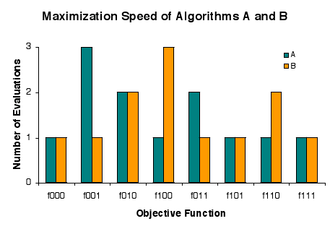
\includegraphics[width=0.5\textwidth]{./assets/freemeal.png}
  \caption{Сравнение предел централизации и придела децентрализации}
  \label{fig:free-meal}
\end{figure}

В итоге анализ приводит к выводу, что компромиссах между скоростью реакции, прозрачностью, нейтральностью и надёжностью. Любая «средняя» архитектура оказывается либо перегружена централизованным контролем, либо лишена достаточного уровня координации, и не превосходит оба экстремума по совокупности критериев.

Таким образом, механизм должен быть построен таким образом, чтобы учитывать возможность влияния на агентов.

% ## 2.5
\mysection{Вывод по второй главе}

Состоит из трех частей:
\begin{enumerate}
  \item Агент
  \item Среда
  \item Механизм
\end{enumerate}


Верхнеуровневая структура механизма распределения ресурсов представлена на рисунке~\ref{fig:idef0}.

\begin{figure}[h]
  \centering
  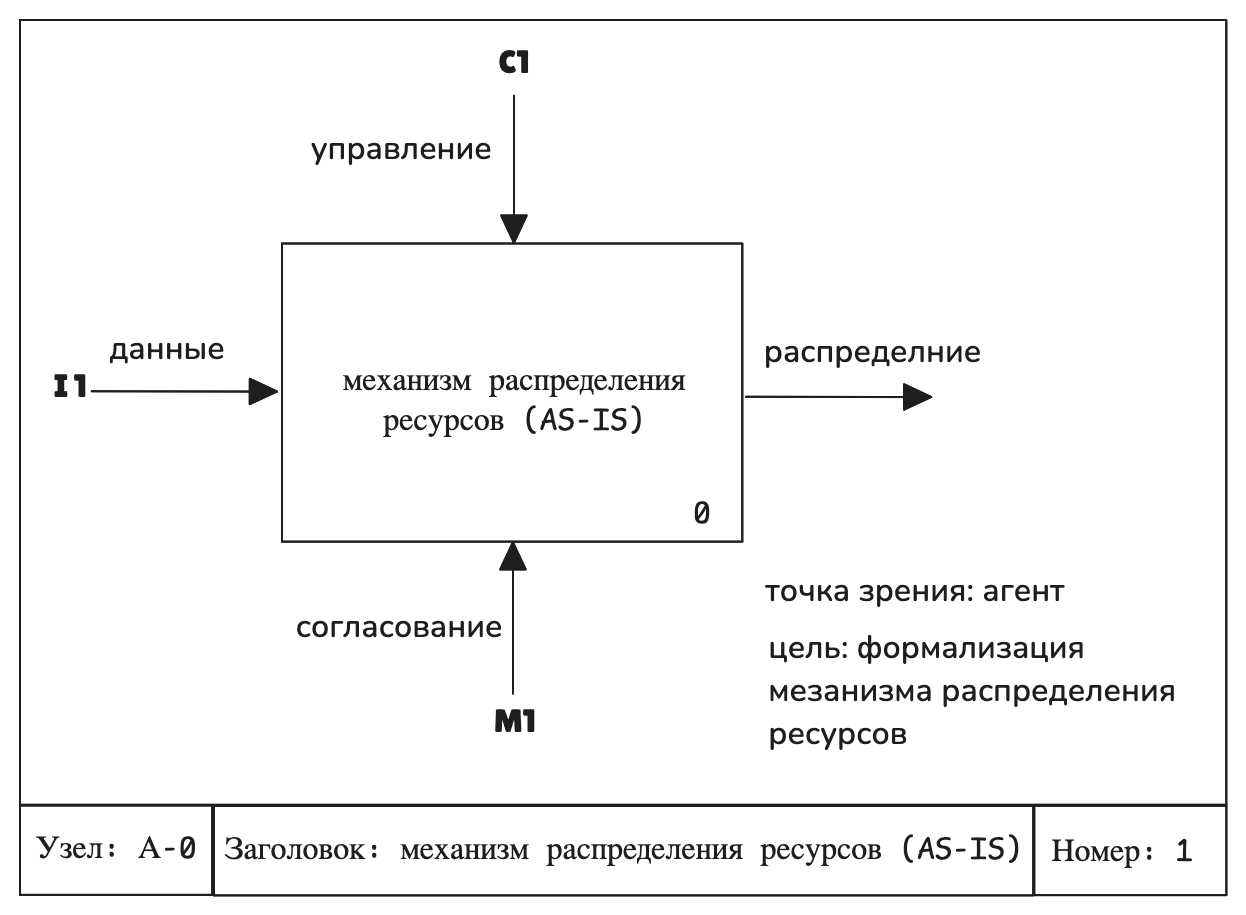
\includegraphics[width=0.9\textwidth]{./assets/idef0-as-is.png}
  \caption{Механизм распределения ресурсов в нотации IDEF0}
  \label{fig:idef0}
\end{figure}

Рассмотрим составные элементы системы:
\begin{enumerate}
  \item Входы (Input) -- данные, частные знания или сигналы окружения необходимые для выполнения функции.
  \item Управление (Control) -- правила, политики или условия, управляющие функцией.
  \item Выходы (Output) -- результаты выполнения функции.
  \item Механизмы (Mechanism) -- стимулы для добровольного участия и согласования локальных решений в единую глобальную норму.
\end{enumerate}

Рассмотренная модель демонстрирует, что при корректной настройке стимулов и доверенного центра согласования можно получить систему, способную адаптироваться к изменениям среды и масштабироваться за счёт множества заинтересованных агентов. Условием успеха является обеспечение вероятности правильных оценок каждого участника выше 50\%, что гарантирует надёжность принятия решений большинством и по цепочкам зависимостей. Аналогичные принципы уже лежат в основе блокчейн-экосистем, где участники, действуя в собственных интересах, стабильно поддерживают целостность и актуальность распределённого реестра.

% #####################################################
% Глава 3
\mychapter{ИНВЕСТИЦИОННОЙ ОЦЕНКА ЧЕРАЗ МАСШТАБИРОВАНИЕ МОДЕЛИ}
% #####################################################

% ## 3.1
\mysection{Формализация предметной области}

Описанная в предыдущей главе модель распределения ресурсов может быть масштибирована за счет того, что каждый из агентов будет заинтересован в том, чтобы максимизировать свою прибыль.

Консенсус наследуется от блокчейнка
В качестве агента мы буделм использовать пользователей.
Инвесторы и авторы доверяют друг другу и не могут манипулировать механизмом.

Пусть имеется конечный набор проектов \(P=\{p_{1},\dots ,p_{n}\}\) где
каждому проекту \(p_{i}\) требуется вложение капитала объёмом \(C_{i}\).
Также задано множество независимых участников \(A=\{a_{1},\dots ,a_{m}\}\).
Участник \(a_{j}\) может вложить сумму \(c_{ij}\ge 0\) в проект \(p_{i}\).
В ответ он получает выпущенные токены объёмом \(t_{ij}\), причём
\(t_{ij}\) пропорционален внесённому вкладу \(c_{ij}\).
Совокупный объём доступных для распределения средств обозначим через \(M\).

Задача механизма — распределить \(M\) так, чтобы максимизировать
суммарную выгоду участников системы, описываемую функцией
\(U\colon P\times A\to\mathbb{R}\), и одновременно  и одновременно гарантировать соблюдение механизма, изложенного в предыдущей главе. Экономический смысл такого механизма состоит в том, чтобы направлять
ресурсы именно к тем проектам, чья ожидаемая общественная ценность
максимальна, при этом балансируя интересы инвесторов и авторов проектов.

% ## 3.2 У
\mysection{Создание RL модели}

Адаптация параметров механизма во времени реализована отдельным компонентом, который может быть офф-чейн скриптом или сервисом, взаимодействующим с блокчейном. Он периодически собирает данные о системе (объем инвестиций, количество участников, частоту отклоняющихся голосов, случаи потерь stake, волатильность цены токена и т.д.), обновляет состояние для модели и принимает решение, нужно ли скорректировать параметры $\alpha, r, \tau, L$ или размер вознаграждений/штрафов. Такой модуль можно рассматривать как агента, действующего в среде, состояние которой – это текущее состояние платформы, а действия – это установка новых значений параметров. Цель агента – максимизировать некоторый кумулятивный рейтинговый показатель $R_t$ системы (например, метрику устойчивости и эффективности). Мы можем задать задачу как поиск оптимальной политики $\pi^*$, выбирающей действие $a_t$ (набор параметров) на каждом шаге $t$, чтобы максимизировать дисконтированную сумму наград $\sum \gamma^t R_t$ с коэффициентом дисконтирования $0<\gamma<1$. Формально, агент решает задачу оптимизации:

\[
  \pi^* = \arg \max_{\pi} E_{\pi} \left[ \sum_{t=0}^{\infty} \gamma^t R_t \right],
\]

Целевая функция, таким образом, стимулирует RL-модуль находить баланс между свободой инвестирования и необходимыми ограничениями, минимизируя потенциальную выгоду атакующих стратегий.

Для решения этой задачи применяется алгоритм обучения с подкреплением. Мы можем использовать метод политики градиента либо Q-обучения. В силу непрерывного (или достаточно большого дискретного) пространства действий и необходимости стабильности, в реализации удобен подход актор-критик или метод проксимальной оптимизации политики (PPO) \cite{Schulman2017}. Ниже приведён псевдокод на Python, демонстрирующий использование библиотеки Stable-Baselines3 для обучения RL-агента на кастомной среде (см. листинг~\ref{lst:rlmodel}).

Код алгоритма RL представлен в листинге \ref{lst:rlmodel}.

\begin{lstlisting}[language=Python, caption={Пример кода}, label={lst:rlmodel}]
  def example_function():
      return "Hello from Listing"
\end{lstlisting}

% ## 3.3
\mysection{Экономическое обоснование}

\mysubsection{Augmented Bonding Curve (ABC)}

Для динамического ценообразования токена проекта $p_i$ используем
функцию
%
\[
  P_i(s)=\alpha_i\, s^{\beta_i}, \qquad
  \beta_i=\frac{1}{1-r_i}, \; r_i\in(0,1),
\]
%
где $s$~--- текущее количество выпущенных токенов.
При вкладе $c_{ij}$ инвестор $a_j$ получает
\[
  t_{ij} \;=\; \frac{c_{ij}}{P_i\!\bigl(s_{\text{prev}}\bigr)},
\]
что уточняет ранее введённое условие пропорциональности
$t_{ij}\propto c_{ij}$.
Таким образом, ABC связывает размер выпуска с резервом
и делает цену токена функцией совокупного предложения
\cite{Zargham2019}.

\mysubsection{Quadratic Funding (QF)}

Софинансирование из общего пула $M$ определяется правилом
\[
  M_i \;=\; \Bigl(\sum_{j}\sqrt{c_{ij}}\Bigr)^2
  \quad\Longrightarrow\quad
  \tilde{C}_i \;=\; \sum_{j} c_{ij}+M_i ,
\]
где $\tilde{C}_i$~--- эффективный объём капитала проекта.
QF изменяет целевую функцию полезности:
\[
  U(p_i,A)\;\longrightarrow\;
  U^{\text{QF}}(p_i,A)
  \,=\,U\!\bigl(\tilde{C}_i,A\bigr),
\]
усиливая влияние массовой поддержки


% ## 3.?.1
\mysubsection{Proof of Stake (PoS)}

Каждый валидатор вкладывает залог $s_j$.
Обновление залога по итогам раунда оценки задаётся правилом
\[
  s_j' \;=\;
  \begin{cases}
    s_j(1+\rho),   & \text{прогноз верен},   \\[4pt]
    s_j(1-\sigma), & \text{прогноз неверен},
  \end{cases}
\]
где $\rho\ge 0$ и $0\le\sigma\le 1$.
Потенциальный штраф $\sigma s_j$ вводит
стоимость атаки Сибилла и
модифицирует индивидуальную полезность агента:
\[
  U_j^{\text{PoS}}
  \,=\,U_j-\sigma s_j .
\]
Тем самым PoS защищает формулу распределения средств
от манипуляций идентичностями
\cite{Kiayias2017}.

\mysubsection{Reinforcement Learning (RL)}

Алгоритм RL рассматривает состояние
$s_t=\bigl(\alpha_i,r_i,\tilde{C}_i,\text{метрики поведения}\bigr)$
и выбирает действие
$a_t=\bigl(\Delta\alpha_i,\Delta r_i,\Delta\tau_i,\Delta L_i\bigr)$,
обновляя параметры ABC и сопутствующие коэффициенты:
\[
  (\alpha_i,r_i,\tau_i,L_i)\;\gets\;(\alpha_i,r_i,\tau_i,L_i)+a_t .
\]
Оптимальную стратегию
\(
\pi^*=\arg\max_\pi\mathbb{E}_\pi
\bigl[\sum_{t}\gamma^t R_t\bigr]
\)
обучаем так, чтобы величина $R_t$ отражала рост
$U^{\text{QF}}(p_i,A)$ и снижение числа нарушений,
что адаптивно корректирует саму формулу $P_i(s)$
и связанное с ней распределение токенов.

% ## 3.3
\mysection{Оптимизационная стратегия}

Основной уязвимостью QF являются Sybil-атаки, устранение которых реализовано по аналогии с помощью меранизма proof of stake \cite{} создающим экономический барьер для многочисленных фейковых аккаунтов.

Почему нельзя обмануть систему? \cite{nakamoto2008bitcoin}

Согласно теории игр, описанный механизм приводит систему к динамическому равновесию Нэша \cite{nash1951non}, в котором ни одному агенту не выгодно отклоняться от честного поведения. Каждый агент ставит часть капитала (stake), рискуя им при оценке проекта. Если его прогноз согласуется с коллективным результатом, ставка возвращается с прибылью, иначе частично или полностью теряется. Таким образом, рациональный агент мотивирован действовать честно и использовать всю доступную ему информацию.

Дополнительно реализован механизм на основе Reinforcement Learning (RL), который адаптивно настраивает параметры токеномики (например, коэффициенты ABC и требования по ставкам), минимизируя возможности для манипуляций и усиливая стимулы к честной игре:
\[
  \pi^* = \arg\max_{\pi} \mathbb{E}\left[\sum_{t=0}^{\infty} \gamma^t R_t\right].
\]

\begin{figure}[h]
  \centering
  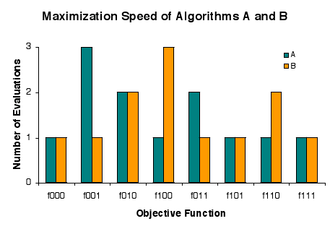
\includegraphics[width=0.5\textwidth]{./assets/freemeal.png}
  \caption{Сравнение предел централизации и придела децентрализации}
  \label{fig:freemeal}
\end{figure}

% ## 3.4
\mysection{Реализация смарт-контракта}

Индивидуальному агенту не выгодно нарушать правила, и выгодно совершать полезную работу по оценке стартапов (предсказывать)

Этот принцип был описан в работе \cite{nakamoto2008bitcoin}

\begin{figure}[h]
  \centering
  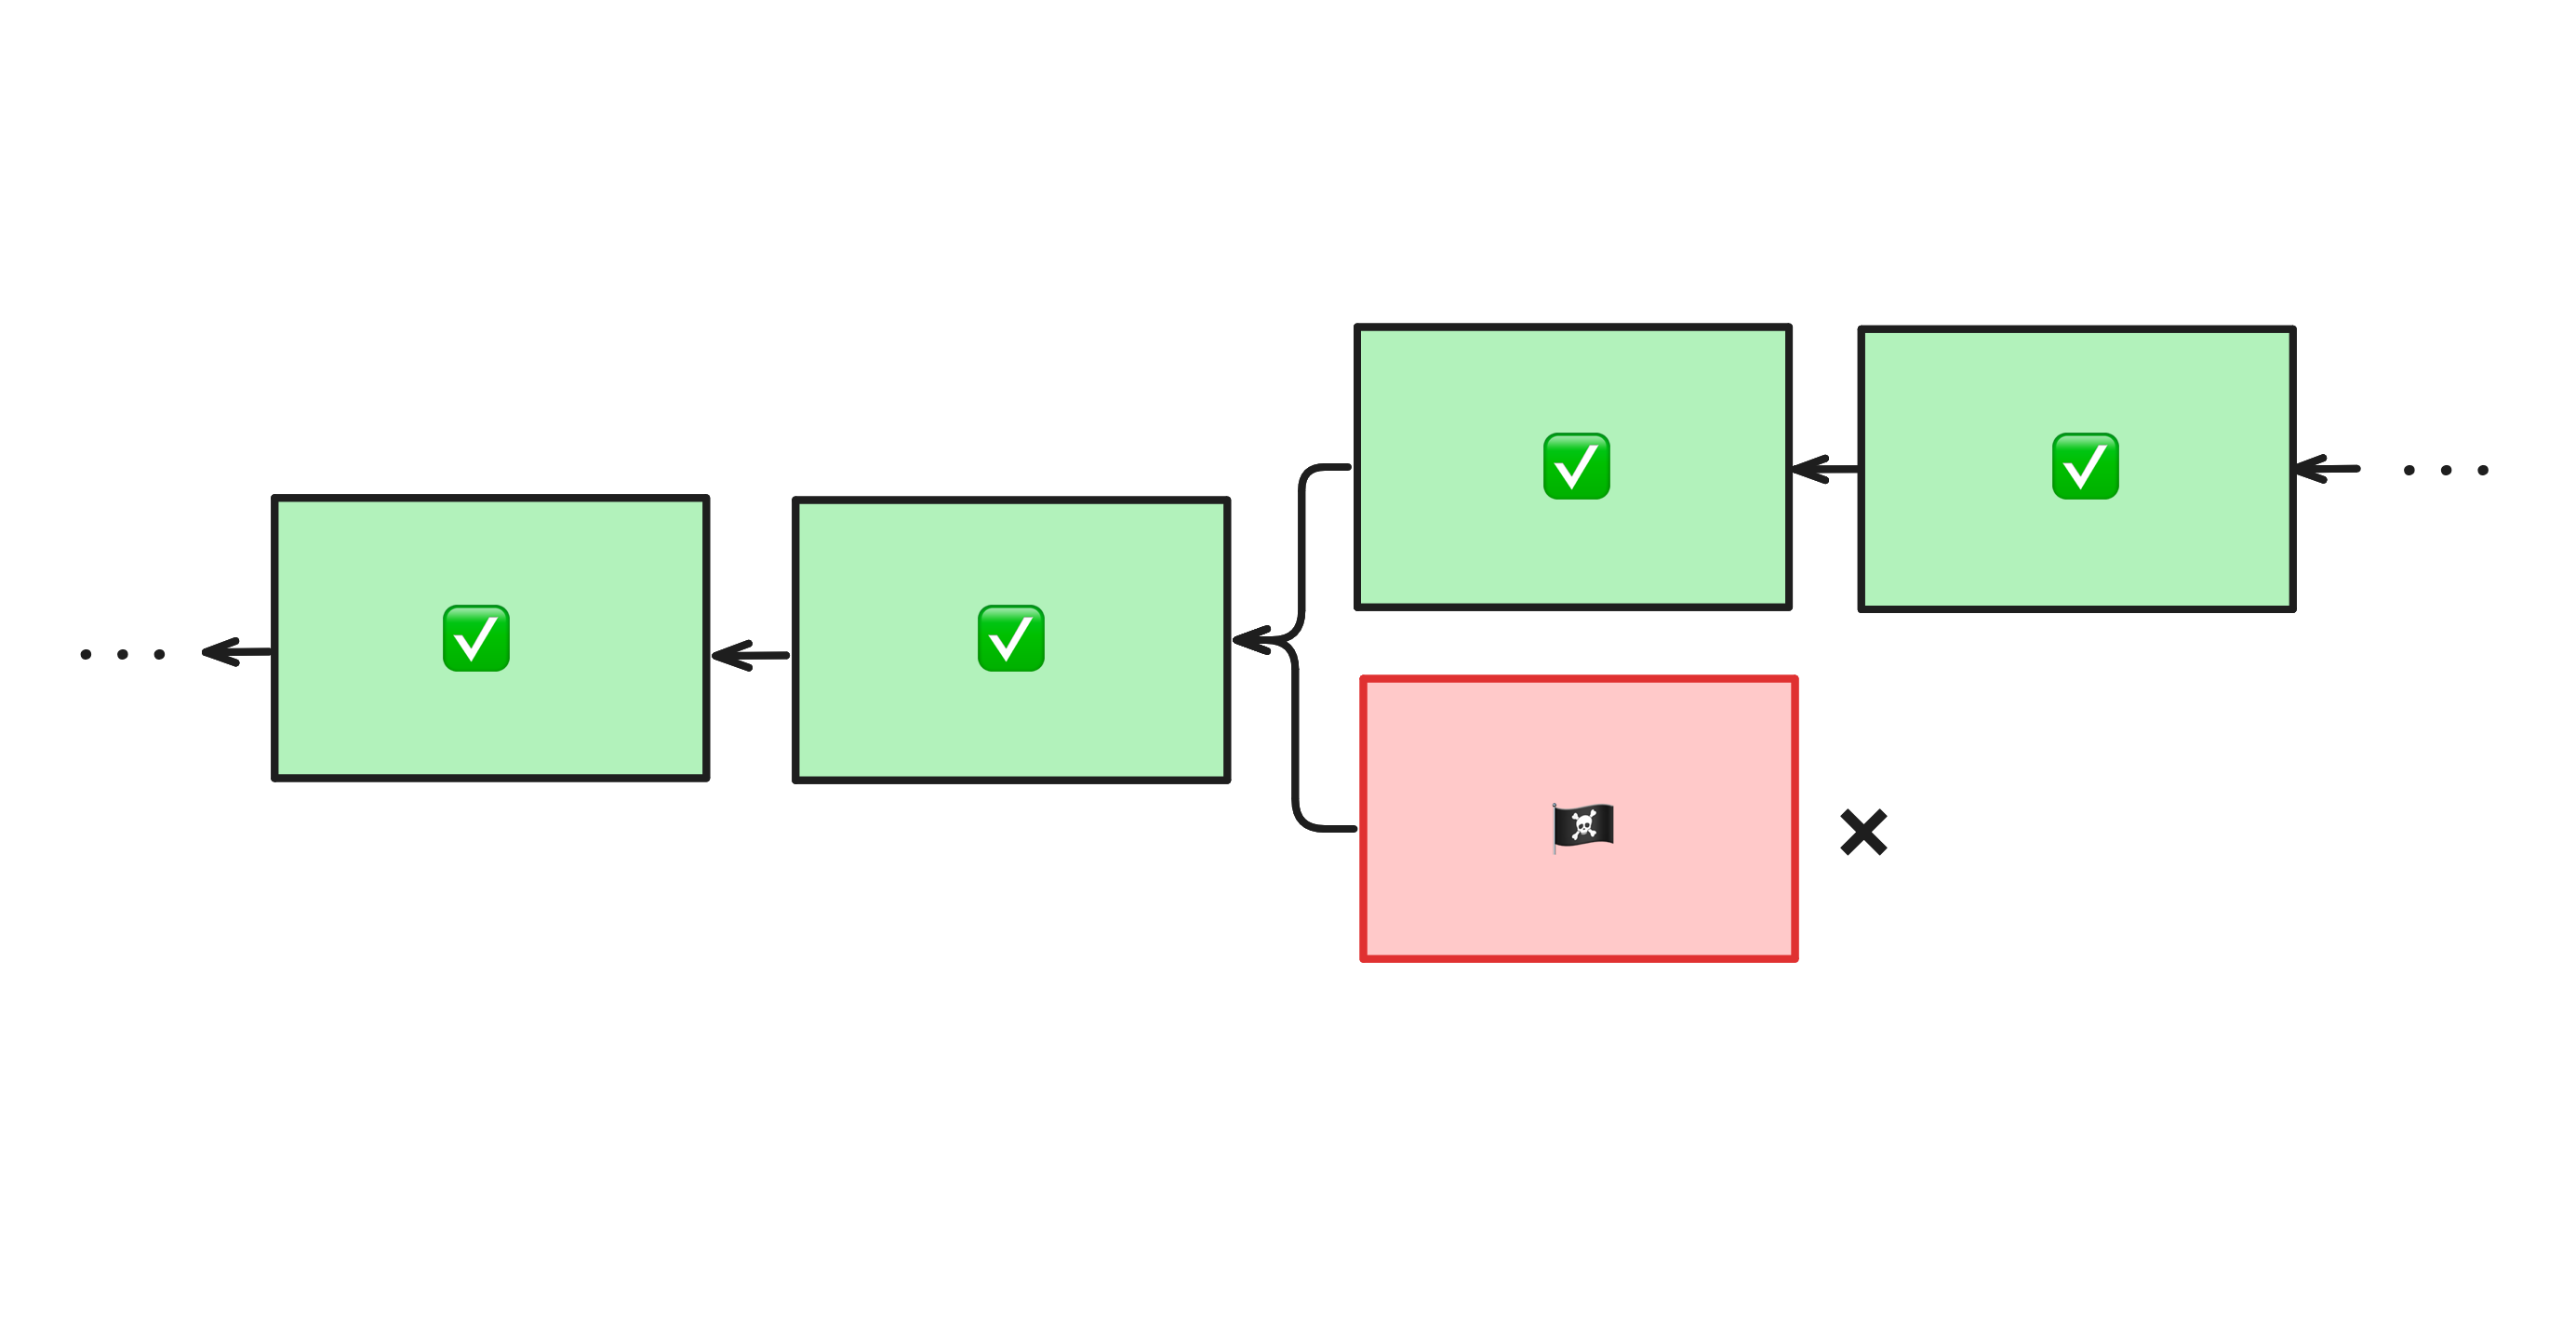
\includegraphics[width=0.9\textwidth]{./assets/longest-chain.png}
  \caption{Longest chain grows the fastest}
  \label{fig:longest-chain}
\end{figure}

У участников системы есть скрытые знания о стартах, которые они мотивированы применить, чтобы забрать награду.

Почему я создаю изолированную систему: Новые идеи не подвержены скрытым знаниям (Y), что помогает не искажать модель.

Тк в системе создаются новые идеи без скрытых знаний это не будет влиять оценку агентов. Но в перспективе данную модель можно использовать при реальном рыночном анализе, где значения X и могут быть манипулированы.

Общеизвестная теорема Кондорсе о жюри \cite{condorcet1785essay} утверждает, что если каждый агент делает правильные прогнозы с вероятностью чуть выше 50\%, то точность коллективного решения экспоненциально растёт с увеличением количества агентов.

Индивидуальный инвестор ограничен собственной неполной информацией и когнитивными искажениями. Однако группа агентов, действующая без скоординированных манипуляций, эффективно агрегирует частичную информацию, формируя более точное представление о перспективности стартапа.

% Экспоненциальный рост точности прогнозов согласно теореме Кондорсе.

Для обеспечения стимулов к честной игре и защиты от манипуляций, в системе реализован механизм Proof of Stake (PoS) \cite{king2012ppcoin},

Токенизацией через Augmented Bonding Curve (ABC) и механизмом Quadratic Funding (QF). Кривая ABC определяется формулой:
\[
  P(s) = \alpha \cdot s^\beta, \quad \beta = \frac{1}{1-r}, \quad r \in (0,1),
\]
где $s$ — текущее количество выпущенных токенов, $\alpha$ — масштабный коэффициент, а $r$ — резервный коэффициент. QF распределяет финансирование из общего пула на основе квадратичной функции индивидуальных вкладов:
\[
  M_i = \left(\sum_j \sqrt{c_{ij}}\right)^2,
\]
обеспечивая преимущество массовой поддержки над единичными крупными вкладами.

% Иллюстрацию механизма ABC+QF с примерами распределения финансирования.

\begin{figure}[h]
  \centering
  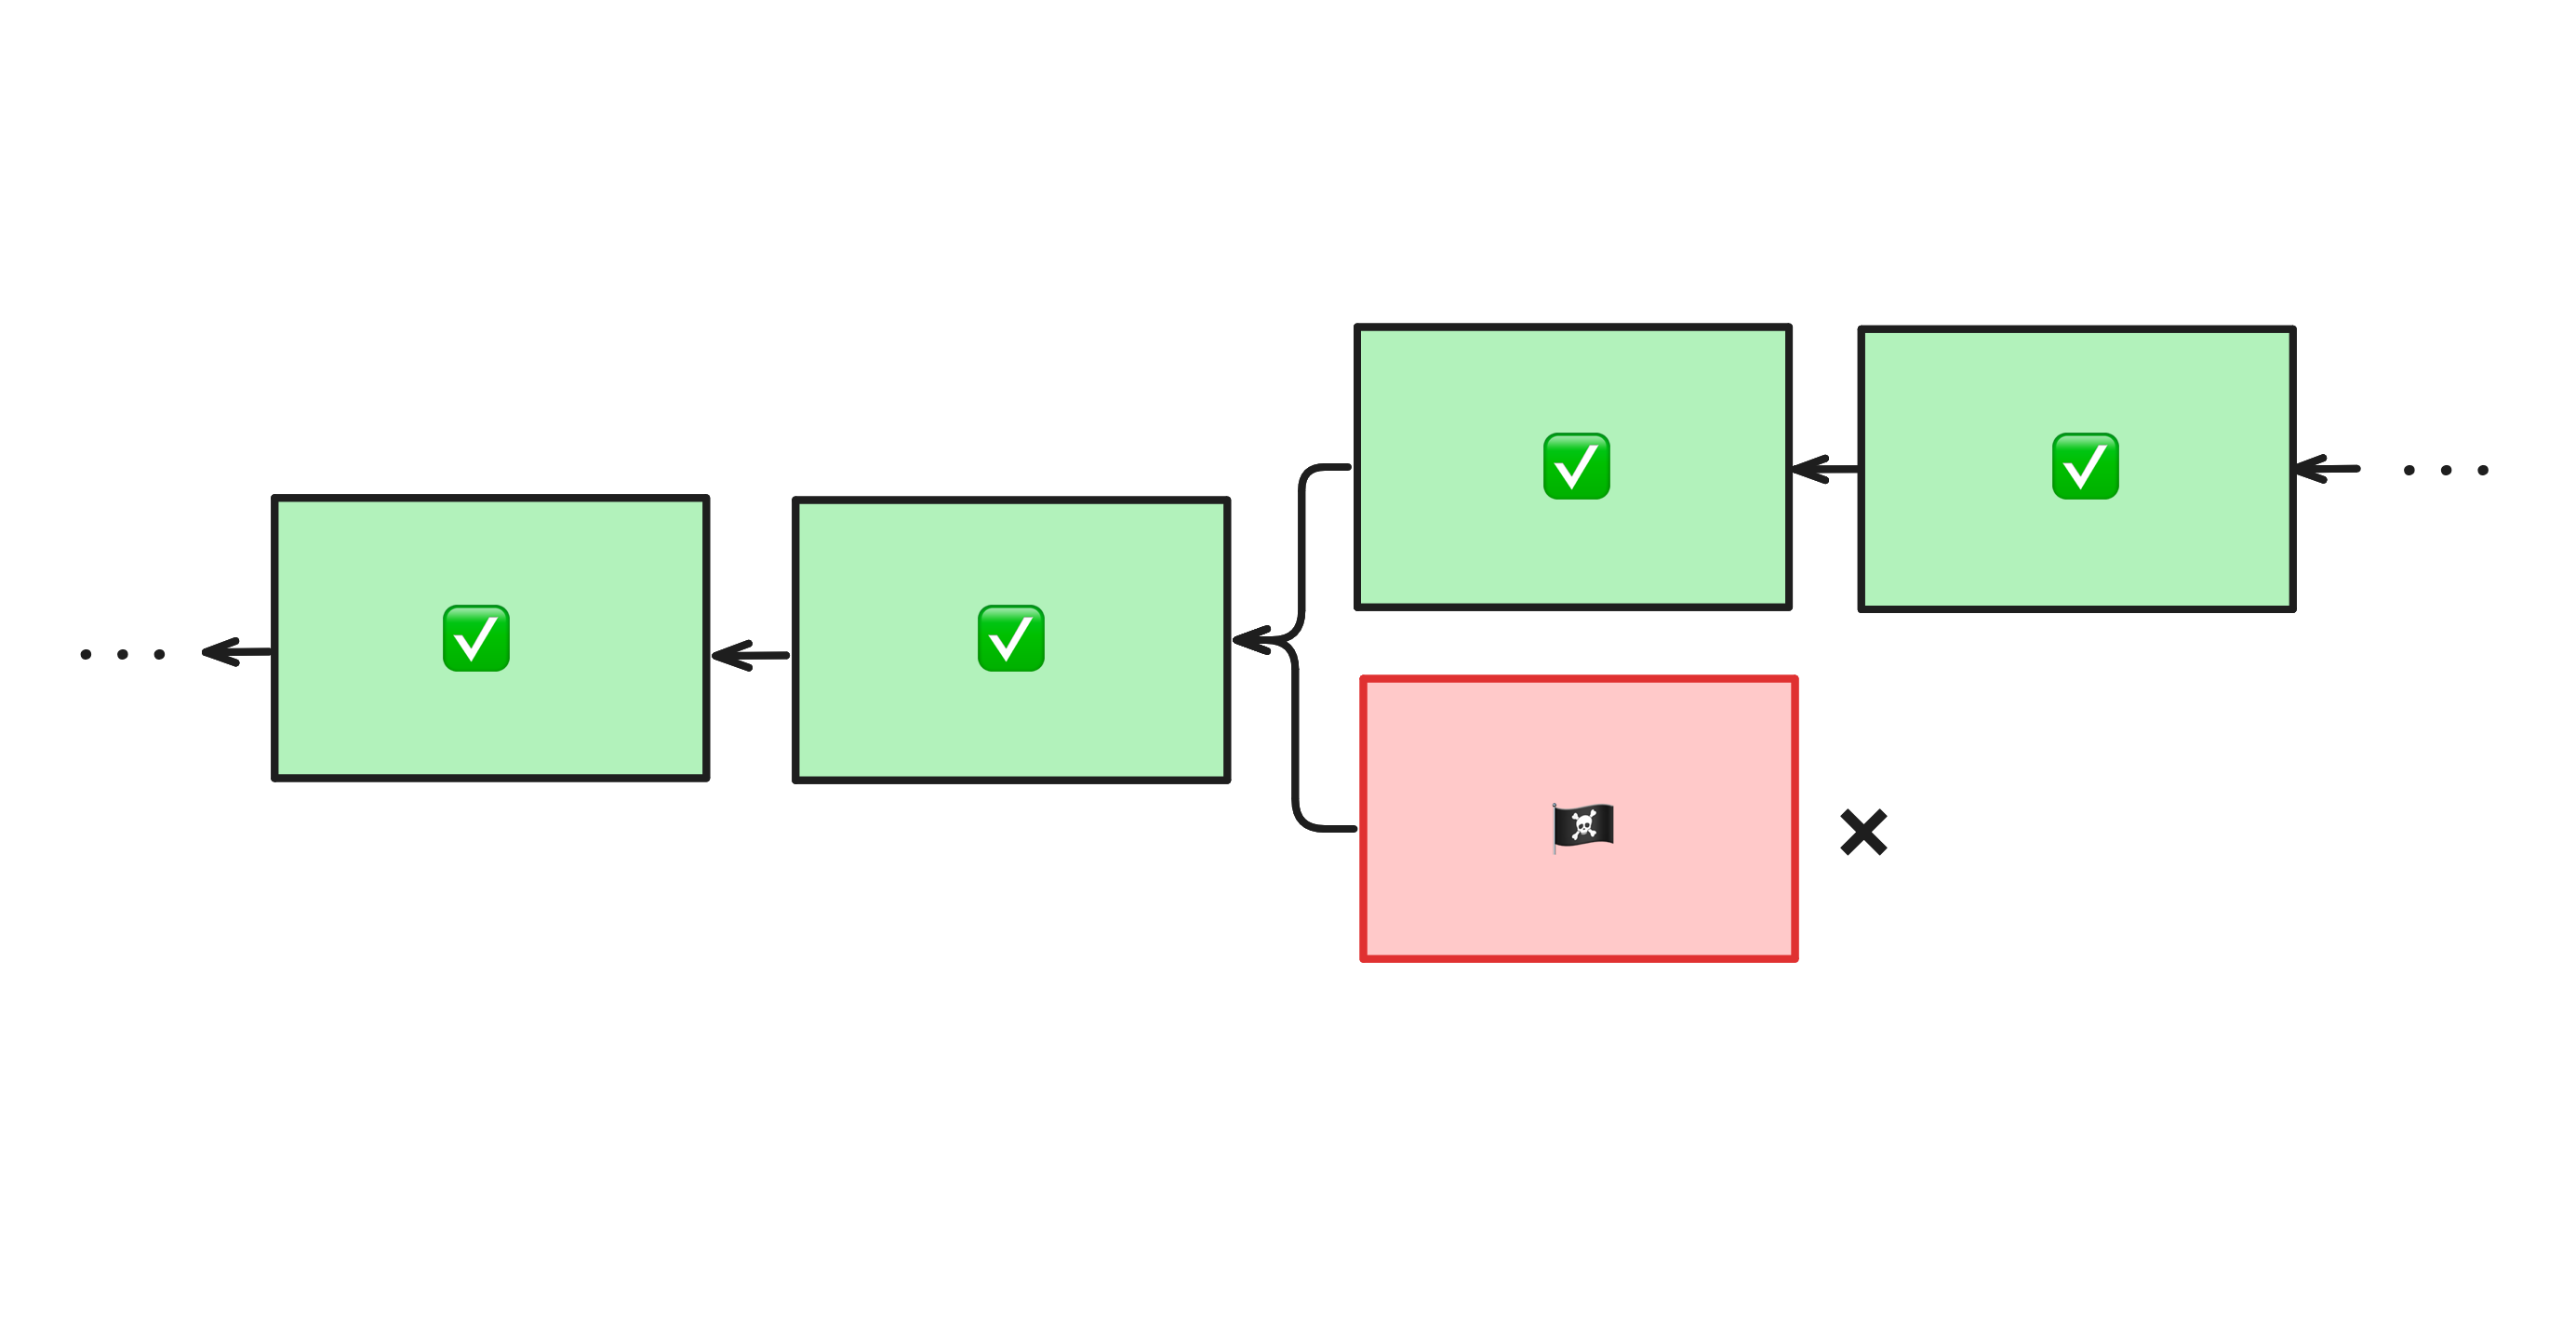
\includegraphics[width=0.9\textwidth]{./assets/longest-chain.png}
  \caption{Longest chain grows the fastest}
  \label{fig:longest-chain}
\end{figure}

% ## 3.5
\mysection{Вывод по третей главе}

Таким образом, разработан механизм, сочетающий стимулы, рациональность агентов и доверенный механизм согласования, что позволяет эффективно распределять ресурсы на основе коллективных прогнозов.

С практической стороны ангелы-инвесторы предоставляют ликвидность авторам стартапов. В зависимости от результата проекта авторы могут выкупать токены полностью, частично или не выкупать совсем. Инвесторы защищены механизмом частичного возврата инвестиций при провале проекта.

% ###################################################
% ## Глава 4
\mychapter{РАЗРАБОТКА ДЕЦЕНТРАЛИЗОВАННОГО ПРИЛОЖЕНИЯ}
% ###################################################

% ## 4.1
\mysection{Описание бизнес-процессов}

% ### 4.1.3
\mysubsection{UML-модель механизма распределения ресурсов}

Для более наглядного представления модели распределения ресурсов в приложении была разработана UML-диаграмма вариантов использования (use case diagram), представленная на рисунке \ref{fig:uml-use-case-diagram}. Данная диаграмма демонстрирует взаимодействие различных акторов системы и распределение ролей между алгоритмическими и человеческими компонентами.

\begin{figure}[ht]
  \centering
  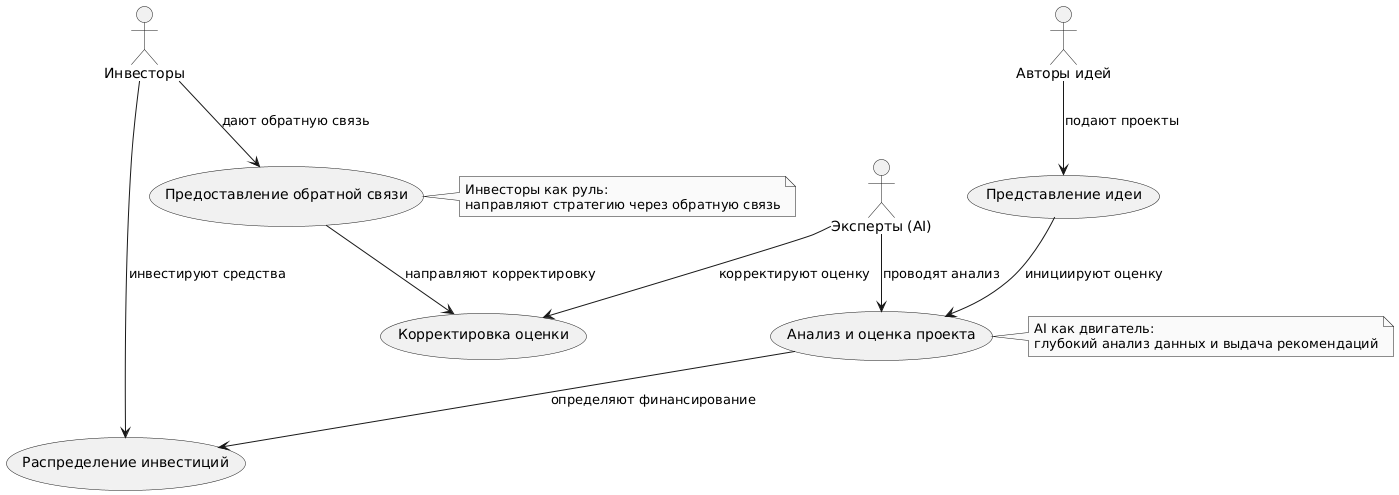
\includegraphics[width=0.9\textwidth]{./assets/uml-use-case-diagram.png}
  \caption{UML-диаграмма вариантов использования механизма распределения ресурсов с балансом автоматизации и человеческого контроля}
  \label{fig:uml-use-case-diagram}
\end{figure}

Как видно из диаграммы, в системе выделяются три основных группы участников: инвесторы, авторы идей и эксперты (представленные, в том числе, системами ИИ). Инвесторы участвуют в процессе предоставления обратной связи и непосредственного инвестирования средств, что направляет стратегию распределения ресурсов. Авторы идей подают свои проекты на рассмотрение через механизм представления идеи. Эксперты, включая аналитические системы на основе ИИ, выполняют ключевую роль по анализу и оценке проектов, а также корректировке предварительных оценок.

Центральными процессами в системе являются:

\begin{enumerate}
  \item Представление идеи -- процесс, при котором авторы формулируют и загружают свои проекты в систему с защитой интеллектуальной собственности.

  \item Анализ и оценка проекта -- основная аналитическая работа по многомерной оценке потенциала проекта, выполняемая в значительной степени автоматизированными системами с глубоким анализом данных.

  \item Предоставление обратной связи -- процесс, в котором инвесторы выражают свои предпочтения и видение направления развития.

  \item Корректировка оценки -- механизм коррекции и уточнения, где эксперты и инвесторы могут скорректировать предварительные результаты анализа.

  \item Распределение инвестиций -- финальный этап, на котором средства распределяются между проектами на основе комплексной оценки, полученной в результате работы механизма.
\end{enumerate}

Особенно важно отметить, что механизм построен по принципу, где алгоритмические компоненты выполняют основную вычислительную работу по обработке больших объемов данных, а человеческие компоненты направляют стратегию через обратную связь, определяют стратегические приоритеты и осуществляют контроль. Такой подход обеспечивает баланс эффективности и надежности, сочетая вычислительную мощь алгоритмов с ценностями и экспертизой человеческих участников.

Данный механизм реализует принцип коллективного принятия решений, где автоматизация используется для обеспечения объективности и масштабируемости, а человеческое участие – для стратегического управления процессом и сохранения этических аспектов распределения ресурсов.

\mysubsection{Процессная модель масштабированного механизма инвестирования}

В целях формализации и визуализации бизнес-процессов функционирования масштабированного механизма инвестирования была разработана BPMN-диаграмма (Business Process Model and Notation), представленная на рисунке \ref{fig:bpmn}. Данная диаграмма иллюстрирует композицию взаимодействий между ключевыми участниками системы и последовательность выполняемых операций в рамках полного инвестиционного цикла.

\begin{figure}[h]
  \centering
  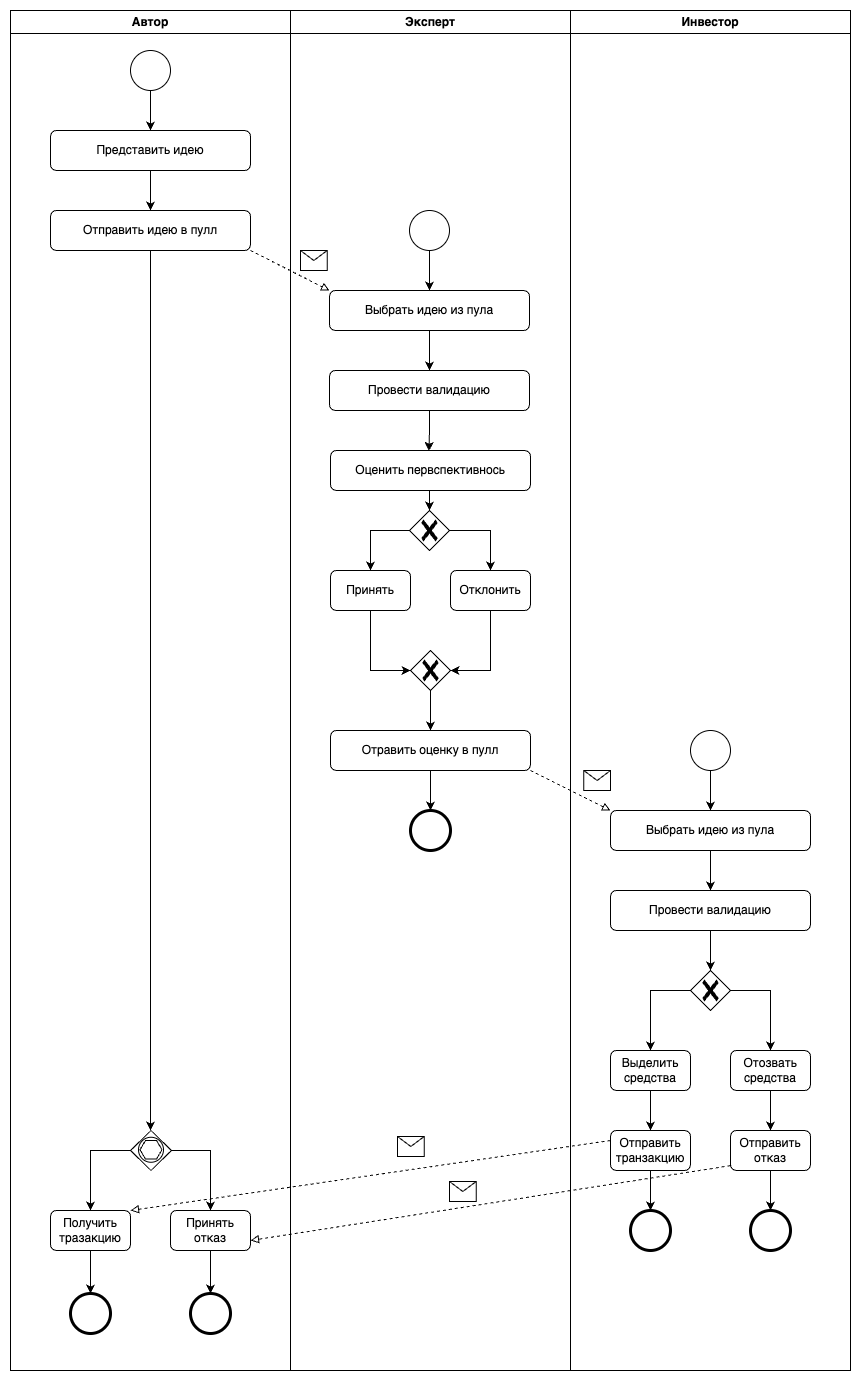
\includegraphics[width=0.5\textwidth]{./assets/bpmn.drawio.png}
  \caption{BPMN-диаграмма процессов масштабированного механизма инвестирования}
  \label{fig:bpmn}
\end{figure}

Информационное взаимодействие между пулом авторов и пулом экспертов осуществляется посредством асинхронных сообщений, что отражает передачу метаданных проекта без раскрытия его полного содержания. В пуле экспертов активируется комплексный подпроцесс, включающий выбор идеи из общего пула, проведение валидации представленных данных и многомерную оценку перспективности проекта. Этот этап реализуется с применением аналитического движка на основе искусственного интеллекта, который обрабатывает структурированные данные проекта с использованием ансамблевых методов машинного обучения. Диаграмма отражает ключевой шлюз (gateway) принятия решения, где эксперт формирует заключение о перспективности идеи на основе результатов аналитического движка и собственной экспертизы. Данное решение может иметь положительный или отрицательный характер, однако в обоих случаях процесс конвергирует к операции отправки оценки в общий пул, что завершает участие эксперта в текущем инвестиционном цикле.

Далее информационный поток направляется к пулу инвесторов, где инициируется подпроцесс выбора и независимой валидации идеи. Центральным элементом данного этапа является шлюз принятия инвестиционного решения, за которым следуют дивергентные пути процесса: выделение средств или отказ от инвестирования. В случае положительного решения активируется последовательность операций финансирования с использованием механизмов квадратичного финансирования и возрастающих кривых ограничения, реализованных посредством смарт-контрактов в выбранной блокчейн-инфраструктуре. При отрицательном решении формируется и отправляется уведомление об отказе.

Заключительный этап процесса визуализируется возвращением информационного потока к пулу автора, где происходит финальное разветвление процесса в зависимости от полученного результата: получение транзакции либо обработка отказа. Оба пути завершаются соответствующими конечными событиями, отражающими завершение инвестиционного цикла для конкретного проекта.

Особого внимания заслуживают интегрированные в диаграмму элементы, отражающие механизмы масштабирования платформы. На уровне технологической инфраструктуры визуализируется применение решений второго уровня (Layer 2) для блокчейна Ethereum, что обеспечивает высокую пропускную способность системы при сохранении базового уровня безопасности. Данный подход позволяет поддерживать растущий объем транзакций без существенного увеличения операционных издержек, что критически важно для развития платформы. Параллельно отображаются процессы мониторинга производительности и автоматического масштабирования вычислительных ресурсов, обеспечивающие адаптивность системы к флуктуирующим нагрузкам.

Диаграмма также отражает ключевые подпроцессы, связанные с обеспечением безопасности и целостности данных, включая распределенное хранение зашифрованной информации в IPFS, применение мультисигнатурных механизмов для критических операций и регулярное резервное копирование состояния системы. Интеграция с внешними сервисами и API визуализируется посредством элементов сервисных задач, подчеркивая взаимодействие системы с внешними компонентами экосистемы.

В контексте управления процессом масштабирования значительную роль играют механизмы обратной связи, позволяющие оперативно корректировать параметры функционирования системы на основе получаемых метрик эффективности. Эти механизмы представлены на диаграмме в виде циклических потоков, соединяющих аналитические процессы с процессами принятия решений о параметрической оптимизации системы.

Таким образом, разработанная BPMN-диаграмма представляет собой комплексное формализованное описание функционирования масштабированного механизма инвестирования, интегрирующее как бизнес-логику взаимодействия ключевых участников, так и технологические аспекты, обеспечивающие масштабируемость, безопасность и адаптивность платформы в условиях возрастающей нагрузки и расширяющегося функционала.

\mysection{Архитектура платформы и основные компоненты}

Архитектура платформы инвестирования разработана с учётом принципов децентрализации, безопасности, масштабируемости, что позволило интегрировать технологии блокчейна, искусственного интеллекта и современные криптографические механизмы в единую систему, способную обеспечить эффективное и справедливое распределение капитала для финансирования инновационных проектов. Данная архитектура построена на модульном принципе, когда различные компоненты, оставаясь взаимосвязанными, функционируют независимо, что обеспечивает гибкость системы и возможность эволюционного развития отдельных её частей. В основе проектирования лежит идея распределения критически важных данных и сервисов по сети, что устраняет единую точку отказа и позволяет обеспечить устойчивость к цензуре, а также применение криптографических методов и принципа минимального необходимого доступа, что гарантирует безопасность и защиту конфиденциальной информации. Кроме того, система сконструирована таким образом, чтобы сохранять высокую производительность при увеличении количества обрабатываемых проектов и пользователей, что достигается за счёт применения решений второго уровня для блокчейна и распределённых вычислений для реализации алгоритмов искусственного интеллекта. Применение открытых стандартов и протоколов способствует созданию интероперабельной среды, а механизмы коллективного управления обеспечивают адаптивность архитектуры к изменяющимся требованиям.

Архитектура приложения представляет собой распределенную систему, включающую фронтенд, бэкенд и вспомогательные сервисы, разворачиваемые посредством CI/CD. Для организации непрерывной интеграции и деплоя применяется GitHub Actions, позволяющий автоматизировать разработческие сценарии, включая сборку и развёртывание приложения
docs.github.com
. На рисунке показан пример уведомления о готовности предварительного просмотра сборки приложения через GitHub Actions (QR-код с ссылкой на предварительный просмотр Expo):

В процессе CI/CD используется GitHub Actions – платформа автоматизации рабочих процессов разработки. GitHub Actions позволяет автоматизировать любые задачи, включая CI/CD, и настраивать сложные последовательности действий
docs.github.com
. При успешной сборке мобильного приложения на платформе Expo в Pull Request автоматически публикуется уведомление с QR-кодом, позволяющее участникам быстро перейти к тестовому билду (см. рис.).

Инфраструктура приложения включает следующие ключевые компоненты и технологии:

\begin{itemize}
  \item React Native (Expo): фреймворк для кроссплатформенной мобильной разработки. На базе Expo построено мобильное приложение, работающее на iOS, Android и в вебе, позволяющее писать универсальный JavaScript-код для пользовательского интерфейса. Expo предоставляет инструменты для быстрой сборки, предварительного просмотра и публикации приложений, упрощая разработку нативных функций (камера, геопозиция и др.). Как отмечается в документации, с помощью Expo можно создавать кроссплатформенные приложения на основе React.

  \item React: библиотека для веб-интерфейса (SPA), обеспечивающая декларативную разработку UI. React позволяет строить интерфейсы «из отдельных частей – компонентов». В нашем веб-клиенте React используется для создания динамического интерфейса, обеспечивающего отзывчивое обновление экрана при изменениях данных.

  \item Telegram Bot: интерфейс обратной связи и модерации, реализованный на Python с помощью библиотеки python-telegram-bot, которая предоставляет асинхронный доступ к Bot API Telegram. Бот используется для приема команд от администраторов (модерация контента, рассылка уведомлений) и взаимодействия с пользователями (обратная связь, уведомления о статусе инициатив).

  \item Telegram Mini Apps: интегрированное веб-приложение внутри мессенджера Telegram позволяют запускать полноценные веб-интерфейсы (HTML/JavaScript) прямо в чате Telegram, обеспечивая «нативный» опыт работы с приложением. С помощью Mini Apps реализован доступ к ключевым функциям приложения (просмотр инициатив, подтверждение решений) без необходимости перехода в отдельное приложение, что улучшает UX и вовлечение аудитории.

\item GitHub Actions: отвечает за сборку и тестирование кода (CI) и автоматическое развёртывание новых версий фронтенда и бэкенда (CD). Настройки рабочих процессов прописаны в YAML-конфигурациях, что позволяет быстро реагировать на изменения в репозитории.

\item IPFS (InterPlanetary File System): используется для распределенного хранения больших файлов и документов (например, материалов инициатив). IPFS – это набор открытых протоколов для адресации, маршрутизации и передачи данных в сети на основе концепции контент-адресации и peer-to-peer передачи docs.ipfs.tech. Благодаря IPFS обеспечивается устойчивое хранение данных вне централизованных серверов.

\item PostgreSQL: реляционная база данных для хранения основной информации (пользователи, инициативы, транзакции, метаданные). PostgreSQL – мощная открытая объектно-реляционная СУБД с более чем 35-летней историей развития, известная своей надёжностью, богатым набором функций и высокой производительностью postgresql.org...(about 7 lines omitted)...react.dev. В нашем веб-клиенте React используется для создания динамического интерфейса, обеспечивающего отзывчивое обновление экрана при изменениях данных.

\item NGINX: веб-сервер и обратный прокси, используемый для балансировки нагрузки и обеспечения защищённого доступа к веб-интерфейсу. NGINX конфигурируется для перенаправления HTTP(S)-запросов к соответствующим сервисам (фронтенд, API) и статического контента.

docs.python-telegram-bot.org
react.dev
docs.telegram-mini-apps.com

\end{itemize}

Базовый уровень архитектуры включает слой блокчейна, отвечающий за запись и верификацию транзакций, исполнение смарт-контрактов и токенизацию активов, а также протокольный слой, в котором реализуются специализированные алгоритмы защиты интеллектуальной собственности, квадратичного финансирования и возрастающих кривых ограничения. Дополнительные слои отвечают за аналитику и обработку данных с использованием искусственного интеллекта, а также за предоставление удобного пользовательского интерфейса, что позволяет участникам системы взаимодействовать с платформой на различных уровнях доступа. При этом интеграция с внешними системами, базами данных и другими блокчейн-платформами расширяет функциональные возможности всей системы.

Ключевые компоненты системы охватывают комплексное управление проектами, инвестиционный механизм, аналитический движок, систему защиты интеллектуальной собственности, платформу децентрализованного управления, а также интерфейсы и API для взаимодействия с внешними сервисами. Функциональность управления проектами реализуется посредством представления и категоризации идей, сопровождаемой механизмами проверки качества и верификации данных, что обеспечивает конфиденциальное взаимодействие между основателями и инвесторами. Инвестиционный механизм базируется на математически обоснованных схемах токенизации и распределения ресурсов, позволяющих оптимизировать финансирование посредством квадратичного механизма и защиты от атак, включая атаки Сибиллы, посредством специально разработанных смарт-контрактов. Аналитический движок, построенный на современных моделях искусственного интеллекта, позволяет проводить комплексный анализ потенциала проектов, оценивать рыночные тренды, выявлять закономерности и прогнозировать успешность проектов. В свою очередь, система защиты интеллектуальной собственности включает в себя современные криптографические протоколы, такие как доказательства с нулевым разглашением, а также механизмы временного закрепления информации на блокчейне и безопасной многосторонней вычислимости. Организация децентрализованного управления посредством DAO, поддерживаемая механизмами голосования и системы репутации, позволяет обеспечить прозрачное и гибкое управление платформой, а разработанные интерфейсы и API делают систему доступной для широкого круга пользователей.

При выборе стека технологий основное внимание уделялось использованию EVM-совместимых блокчейнов для реализации смарт-контрактов, а также решений второго уровня, способствующих повышению масштабируемости и снижению транзакционных издержек. В качестве языков программирования для смарт-контрактов применялись Solidity и Vyper, а разработка сопровождалась использованием проверенных фреймворков, таких как Hardhat и OpenZeppelin. Современные криптографические методы, включая zk-SNARKs и zk-STARKs, обеспечивают защиту конфиденциальной информации, а применение IPFS с шифрованием гарантирует безопасность хранения данных. Реализация алгоритмов искусственного интеллекта осуществлялась на базе фреймворков TensorFlow и PyTorch с применением моделей обработки естественного языка и графовых нейронных сетей, что обеспечивает высокую точность анализа. В серверной части использовались технологии Node.js, Python, GraphQL, Redis и PostgreSQL, а фронтенд разработка осуществлялась с применением React.js и ethers.js, что позволило создать современный и удобный пользовательский интерфейс. Важное значение имели инструменты контейнеризации и оркестрации, такие как Docker и Kubernetes, а также облачные решения, позволяющие обеспечить отказоустойчивость и масштабируемость всей системы.

\mysection{Разработка базы данных}

База данных разработанна как локальная оффчейн-система для мобильного приложения и предназначена для поддержки работы платформы, которая решает задачи инвестирования в ранние стадии стартапов через слепые инвестиции и технологии блокчейна. Центральной таблицей является таблица пользователей, которая содержит информацию о всех участниках платформы — авторах идей (предпринимателях), инвесторах, экспертах и членах сообщества. В этой таблице хранятся уникальные идентификаторы пользователей, их имена, роли (автор, инвестор, эксперт или участник сообщества), электронные адреса и даты регистрации, что позволяет отслеживать взаимодействие каждого участника с платформой. Схема базы даннных представлена на рисуноке \ref{fig:database}.

\begin{figure}[h]
  \centering
  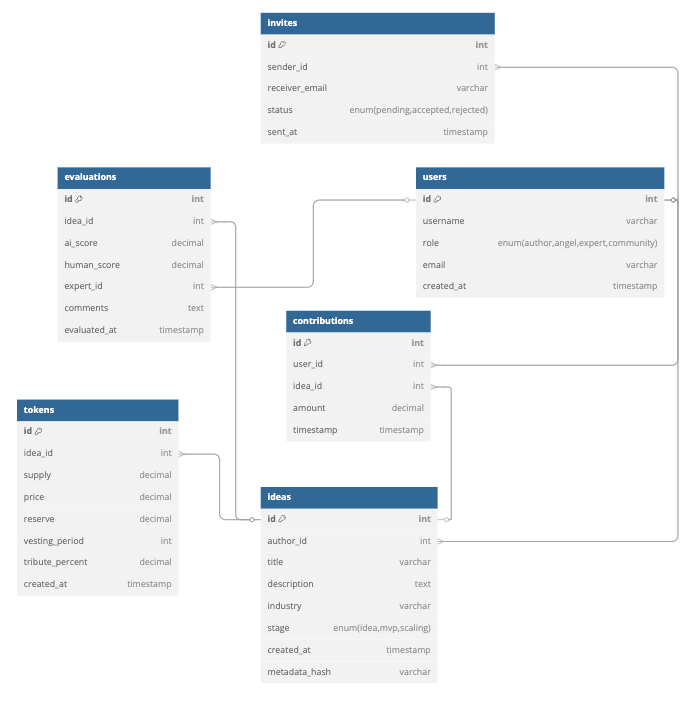
\includegraphics[width=0.5\textwidth]{./assets/database.png}
  \caption{{\protect\hyperlink{fig:database}{Схема базы данных}}}
  \label{fig:database}
\end{figure}

\subsection*{Описание таблиц базы данных}

\mysubsection{Таблица Users}
Хранит информацию о зарегистрированных участниках платформы. Пользователи могут иметь одну из ролей: автор идеи, ангел-инвестор, эксперт или участник сообщества.
\begin{itemize}
  \item \texttt{id} — уникальный идентификатор пользователя
  \item \texttt{username} — имя пользователя
  \item \texttt{role} — роль: author, angel, expert, community
  \item \texttt{email} — адрес электронной почты
  \item \texttt{created\_at} — дата регистрации
\end{itemize}

\mysubsection{Таблица Ideas}
Таблица идей служит для безопасного хранения зашифрованных идей стартапов на устройствах пользователей до момента их токенизации на блокчейне. Она включает уникальные идентификаторы идей, ссылки на авторов из таблицы пользователей, названия и подробные описания идей (зашифрованные для защиты интеллектуальной собственности), а также информацию об отрасли, стадии развития (идея, MVP или масштабирование), дате создания и хеше метаданных, который используется для последующей верификации на блокчейне.
\begin{itemize}
  \item \texttt{id} — уникальный идентификатор идеи
  \item \texttt{author\_id} — внешний ключ на пользователя-автора
  \item \texttt{title} — название идеи
  \item \texttt{description} — описание идеи
  \item \texttt{industry} — отрасль
  \item \texttt{stage} — стадия развития: idea, mvp, scaling
  \item \texttt{created\_at} — дата создания
  \item \texttt{metadata\_hash} — хэш метаданных (например, IPFS)
\end{itemize}

\mysubsection{Таблица Evaluations}
Таблица оценок фиксирует результаты анализа идей, проводимого искусственным интеллектом и людьми, что обеспечивает слепую и объективную оценку для инвестиционных решений.
\begin{itemize}
  \item \texttt{id} — идентификатор оценки
  \item \texttt{idea\_id} — ссылка на оцениваемую идею
  \item \texttt{ai\_score} — оценка ИИ
  \item \texttt{human\_score} — оценка от сообщества
  \item \texttt{expert\_id} — эксперт, проводивший оценку
  \item \texttt{comments} — комментарии к оценке
  \item \texttt{evaluated\_at} — дата оценки
\end{itemize}

\mysubsection{Таблица Contributions}
Таблица вкладов регистрирует локальные финансовые вложения пользователей в идеи до их токенизации на блокчейне. Эта таблица связывает пользователей и идеи, обеспечивая отслеживание финансовой поддержки.
\begin{itemize}
  \item \texttt{id} — уникальный идентификатор транзакции
  \item \texttt{user\_id} — инвестор
  \item \texttt{idea\_id} — финансируемая идея
  \item \texttt{amount} — сумма вклада
  \item \texttt{timestamp} — время вложения
\end{itemize}

\mysubsection{Таблица Tokens}
Таблица токенов управляет локальными данными о токенах, которые будут токенизированы на блокчейне после инвестиций. Таблица связана с таблицей идей, поддерживая механизм распределения ресурсов.
\begin{itemize}
  \item \texttt{id} — уникальный идентификатор токена
  \item \texttt{idea\_id} — связанная идея
  \item \texttt{supply} — объем эмиссии
  \item \texttt{price} — цена токена
  \item \texttt{reserve} — резервный пул
  \item \texttt{vesting\_period} — период вестинга (в днях)
  \item \texttt{tribute\_percent} — трибьют в процентах
  \item \texttt{created\_at} — дата выпуска токена
\end{itemize}

\mysubsection{Таблица Invites}
Таблица приглашений управляет системой инвайтов в сообщество. В ней фиксируются отправители, получатели и текущий статус приглашения.
\begin{itemize}
  \item \texttt{id} — уникальный идентификатор приглашения
  \item \texttt{sender\_id} — отправитель приглашения
  \item \texttt{receiver\_email} — email приглашённого
  \item \texttt{status} — статус: pending, accepted, rejected
  \item \texttt{sent\_at} — дата отправки
\end{itemize}

Важно отметить, что данная структура базы данных используется в контексте модели eventual consistency. Это означает, что согласованность данных между клиентом, сервером и блокчейном достигается не мгновенно, а по мере синхронизации данных, обеспечивая масштабируемость и устойчивость системы к сбоям сетевой инфраструктуры. Такая архитектура особенно эффективна для распределённых децентрализованных приложений, взаимодействующих с внешними источниками данных и блокчейн-сетями.

\mysubsection{Механизм оценки проектов с использованием искусственного интеллекта}

5. Telegram-интеграция и Mini Apps

Такая интеграция расширяет каналы взаимодействия с пользователями: часть функционала доступна напрямую в мессенджере, что упрощает привлечение новой аудитории и ускоряет коммуникацию.

% ## 4.4
\mysection{Разработка серверной части}

В качестве серверного фреймворка в разработанном приложении использовался Fastify — современный, асинхронный и высокопроизводительный веб-фреймворк для Node.js. Он предоставляет поддержку JSON Schema для валидации входящих и исходящих данных, а также встроенные хуки жизненного цикла, плагины, систему маршрутизации и встроенные механизмы сериализации. Благодаря минималистичной архитектуре Fastify, удалось значительно ускорить запуск API и уменьшить накладные расходы при масштабировании.
Для обработки данных и взаимодействия с базой данных применялась PostgreSQL

% ## 4.5
\mysection{Разработка клиентской части}

Интерфейс прототипа разработан с учетом принципов интуитивности и простоты взаимодействия, обеспечивая при этом доступ ко всему функционалу системы.
Общая схема взаимодействия компонентов прототипа представлена на рисунке \ref{fig:app-prototype}, где проиллюстрированы основные процессы и связи между элементами системы.

\begin{figure}[h]
  \centering
  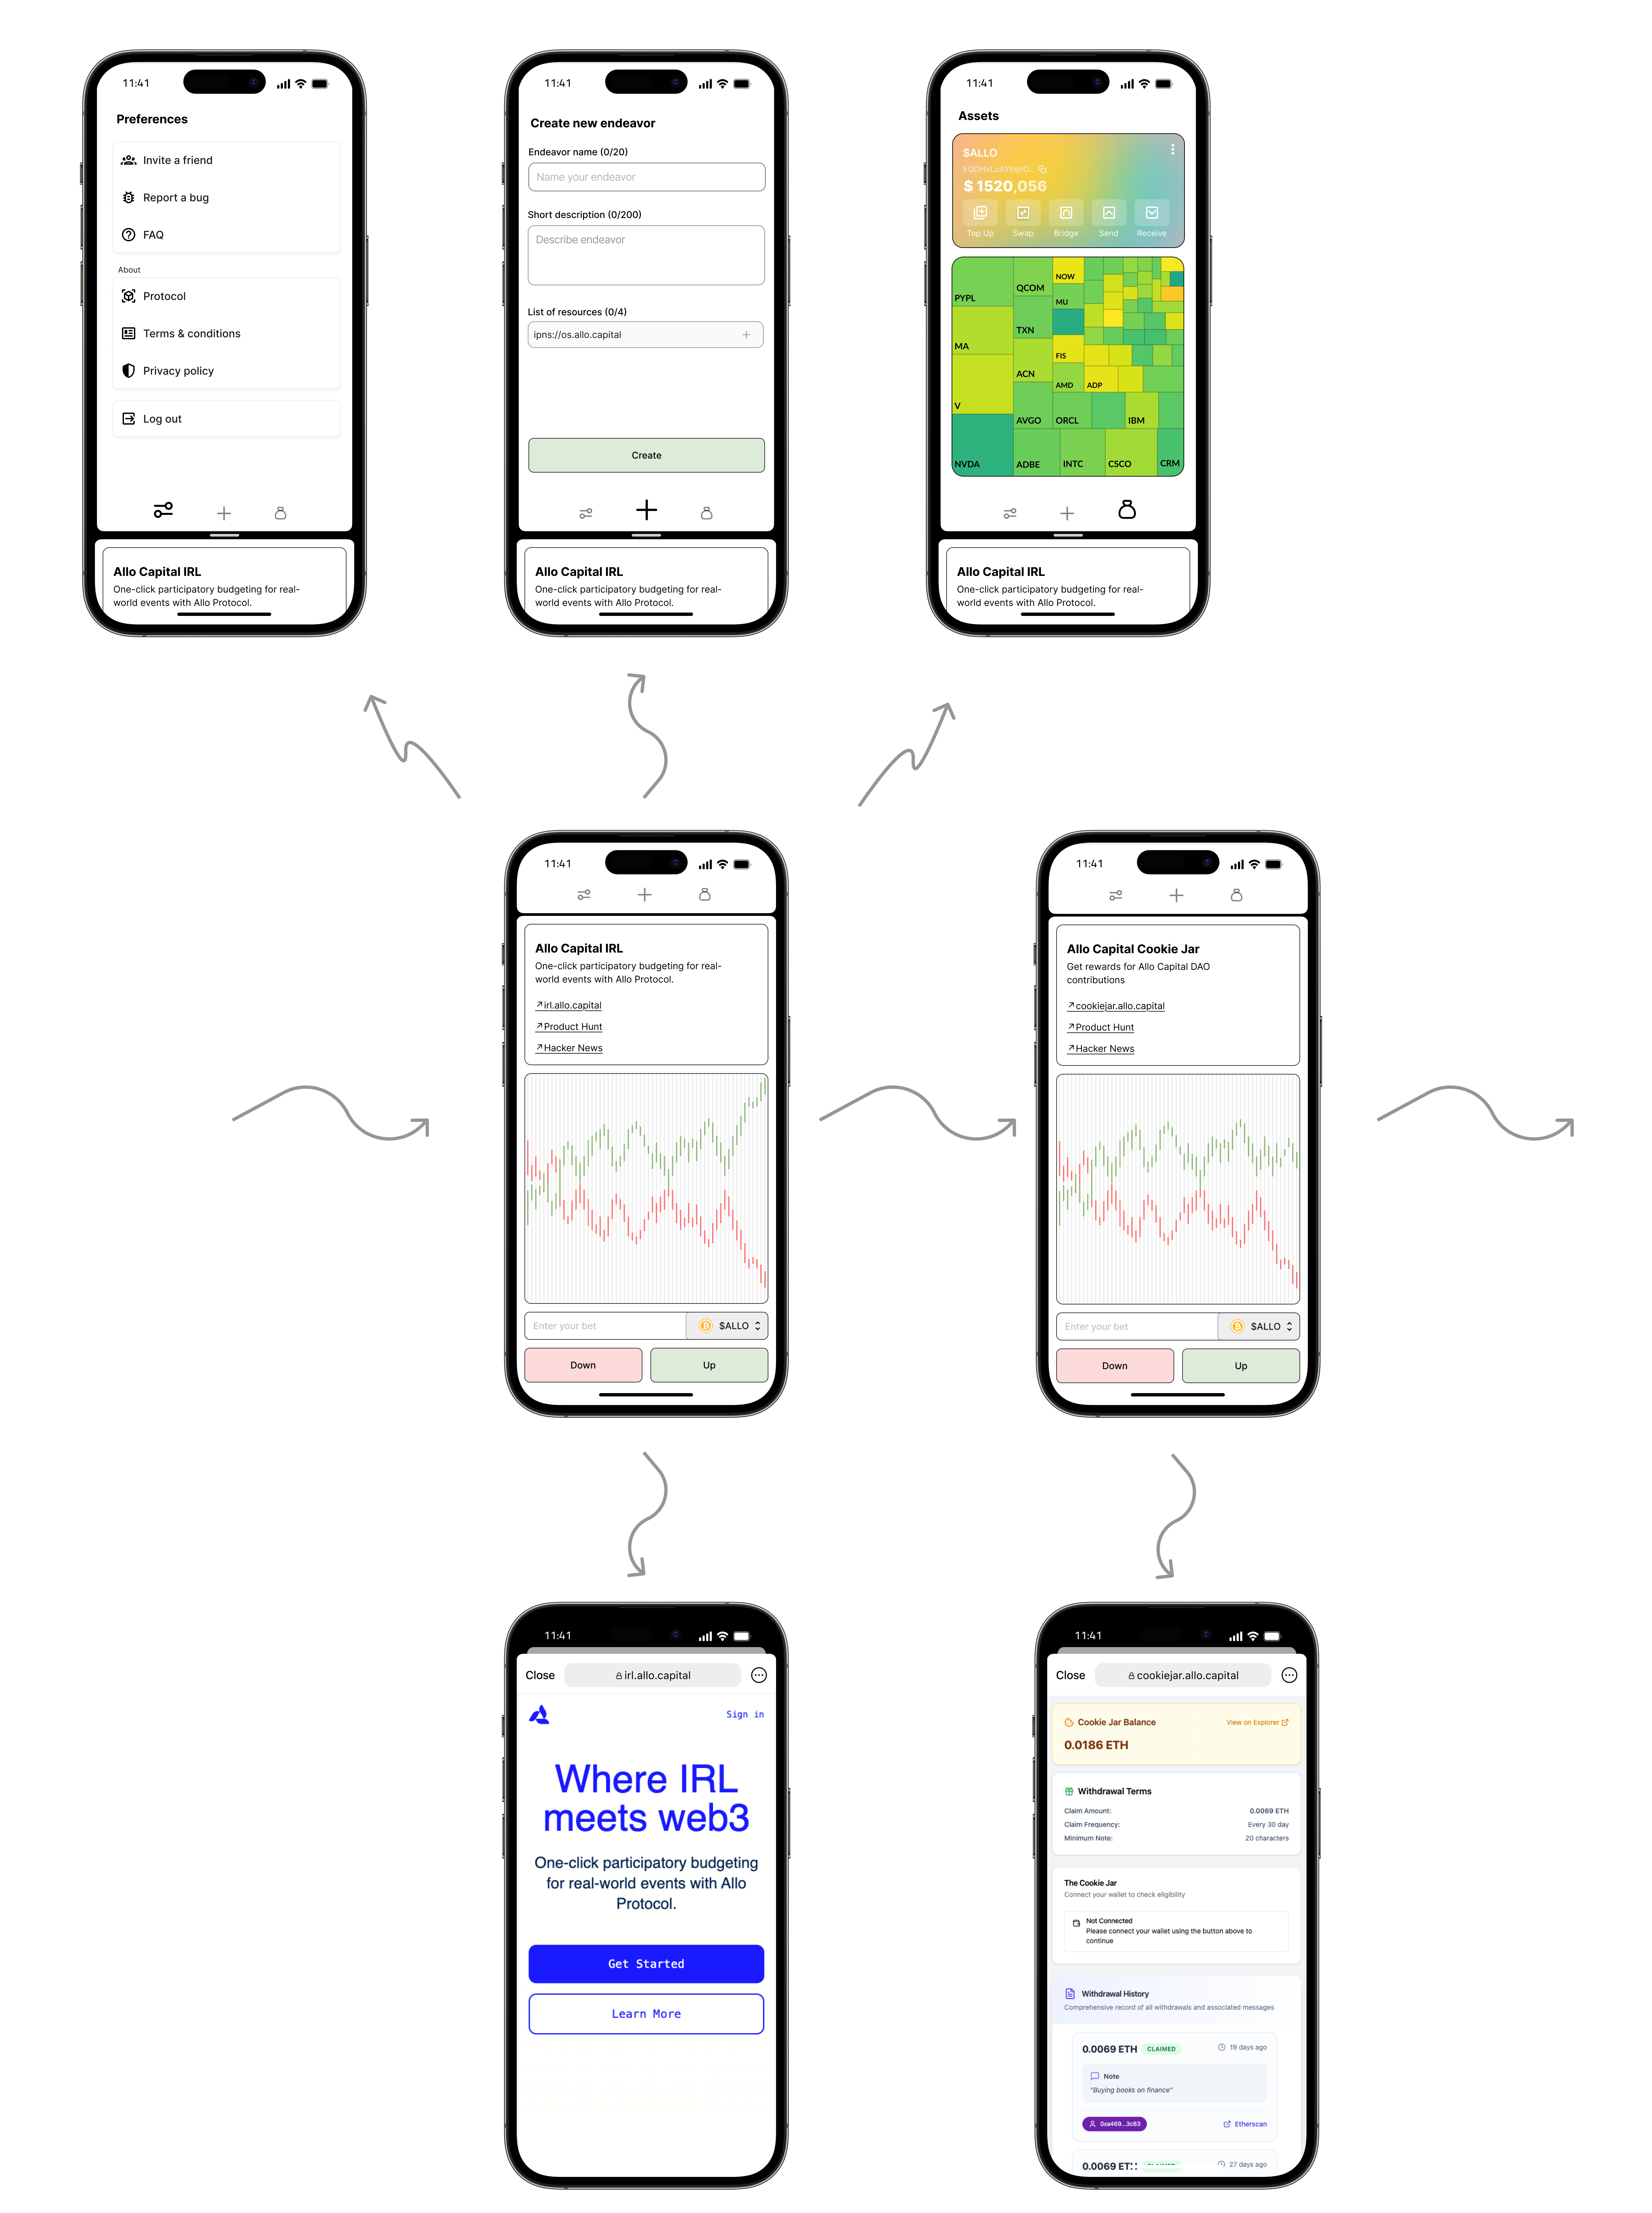
\includegraphics[width=0.5\textwidth]{./assets/app-prototype.png}
  \caption{Схема основных процессов и взаимодействий в прототипе платформы}
  \label{fig:app-prototype}
\end{figure}

% ### 4.5.1
\mysubsection{Главный экран приложения}

Основной сценарий использования приложения. На нём отображается ключевая информация и основные действия, доступные сразу после запуска. В верхней части располагается заголовок приложения или логотип, а также кнопки навигации (например, кнопка меню для перехода к экрану навигации между модулями).

Центральное пространство главного экрана отведено под список текущих инициатив или проектов. Каждая инициатива представлена в виде карточки или строки: содержит название инициативы и её краткое описание. В прототипе на карточке отображается название проекта и одна строка с описанием его цели или сути. Кроме того, под описанием располагаются иконки или ссылки на внешние ресурсы, связанные с этой инициативой (например, иконки Product Hunt или Hacker News, если инициатива упоминается на этих платформах).

Раскрытие лиц увеличивает вероятность успеха инициативы на 3\% \cite{farrel2024leveraging}

Основное назначение главного экрана – предоставить пользователю обзор актуальных инициатив и быстрый доступ к дальнейшим действиям. Пользователь может прокручивать список для просмотра всех доступных инициатив. Нажатие на карточку инициативы приводит к переходу на экран браузера, где раскрываются подробности выбранного проекта в виде встроенной веб-страницы.

С главного экрана также доступен переход к созданию новой инициативы – это реализовано через отдельную кнопку (значок "+" на панели) или через меню навигации. Пример отображения главного экрана приведён на рисунке \ref{fig:app-main-flow}.

\begin{figure}[h]
  \centering
  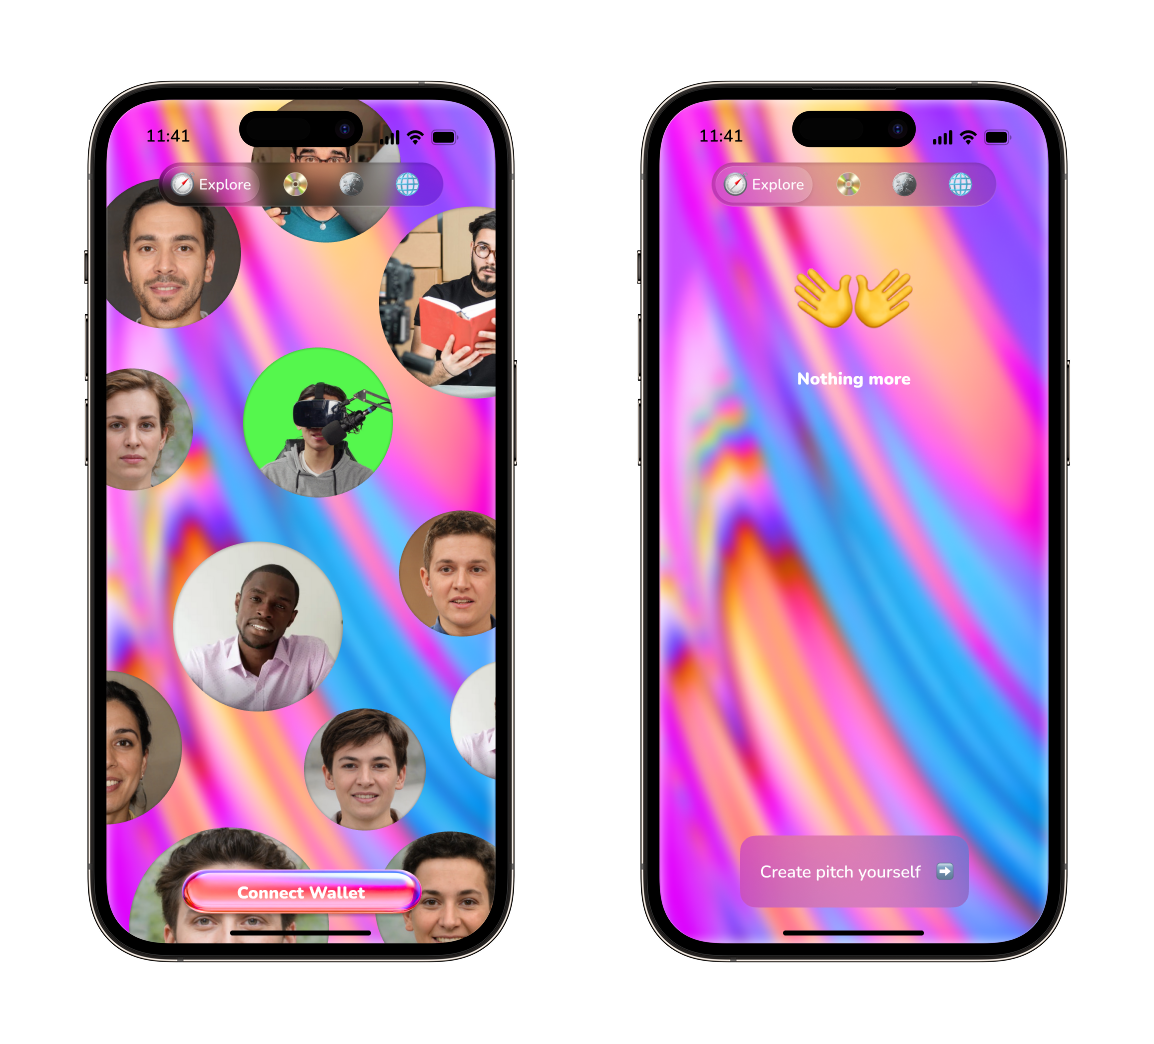
\includegraphics[width=0.5\textwidth]{./assets/app-main-flow.png}
  \caption{Главный экран приложения со списком инициатив}
  \label{fig:app-main-flow}
\end{figure}

\mysubsection{Экран браузера}

Экран браузера предназначен для отображения детальной информации об инициативе посредством встроенного веб-браузера. Этот экран открывается, когда пользователь выбирает инициативу на главном экране или нажимает на связанный с ней внешний ресурс.

В верхней части экрана браузера присутствует панель навигации: она содержит кнопку «Назад» для возвращения к предыдущему экрану (например, обратно к главному списку) и отображает адрес или название ресурса, который просматривается. Основное пространство занимает содержимое веб-страницы, связанной с выбранной инициативой.

В прототипе при открытии инициативы пользователь видит встроенную страницу с подробным описанием проекта: заголовок, расширенное описание, мультимедийные материалы и кнопки взаимодействия (такие как «Get Started», «Learn More»).

Во время просмотра встроенной страницы пользователь может взаимодействовать с ней так же, как в обычном браузере: прокручивать контент, нажимать на ссылки или кнопки. При этом, благодаря встроенному браузеру, нет необходимости покидать приложение. Пример экрана браузера представлен на рисунке \ref{fig:app-browser}.

\begin{figure}[h]
  \centering
  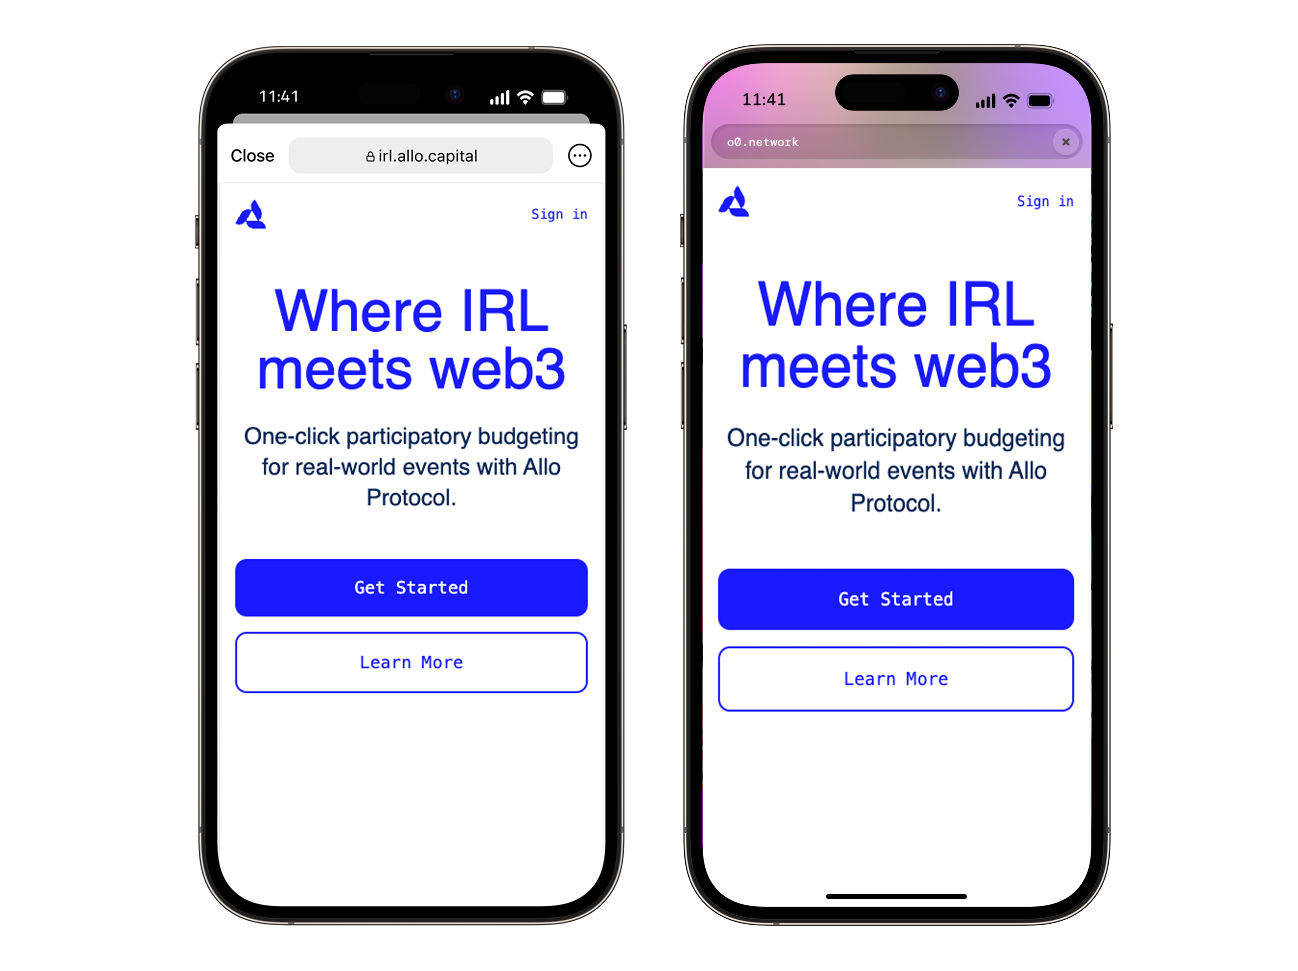
\includegraphics[width=0.5\textwidth]{./assets/app-browser.png}
  \caption{Пример экрана браузера с детальной информацией о проекте}
  \label{fig:app-browser}
\end{figure}

В появившемся меню отображается список пунктов, позволяющих перейти к различным экранам: например, к экрану управления активами, к экрану создания новой инициативы, к профилю или настройкам. В верхней части навигационного меню показывается профиль пользователя (имя, аватар) или название приложения, а ниже перечислены основные разделы.

В прототипе меню навигации содержит пункты: «Assets» (Активы) для перехода к финансовым показателям, «Create new endeavor» (Создать инициативу) для запуска экрана создания проекта, а также ряд пунктов, связанных с настройками пользователя и информацией о системе. Например, в меню присутствуют элементы «Preferences» (Настройки), «Invite a friend» (Пригласить друга), «Report a bug» (Сообщить об ошибке), «FAQ» (Частые вопросы), «About» (О приложении), «Protocol» (Информация о протоколе платформы), «Terms \& conditions» (Пользовательское соглашение), «Privacy policy» (Политика конфиденциальности) и «Log out» (Выход из аккаунта).

Пример экрана навигации показан на рисунке \ref{fig:app-navigation}, где представлены различные модули доступные пользователю.

\begin{figure}[h]
  \centering
  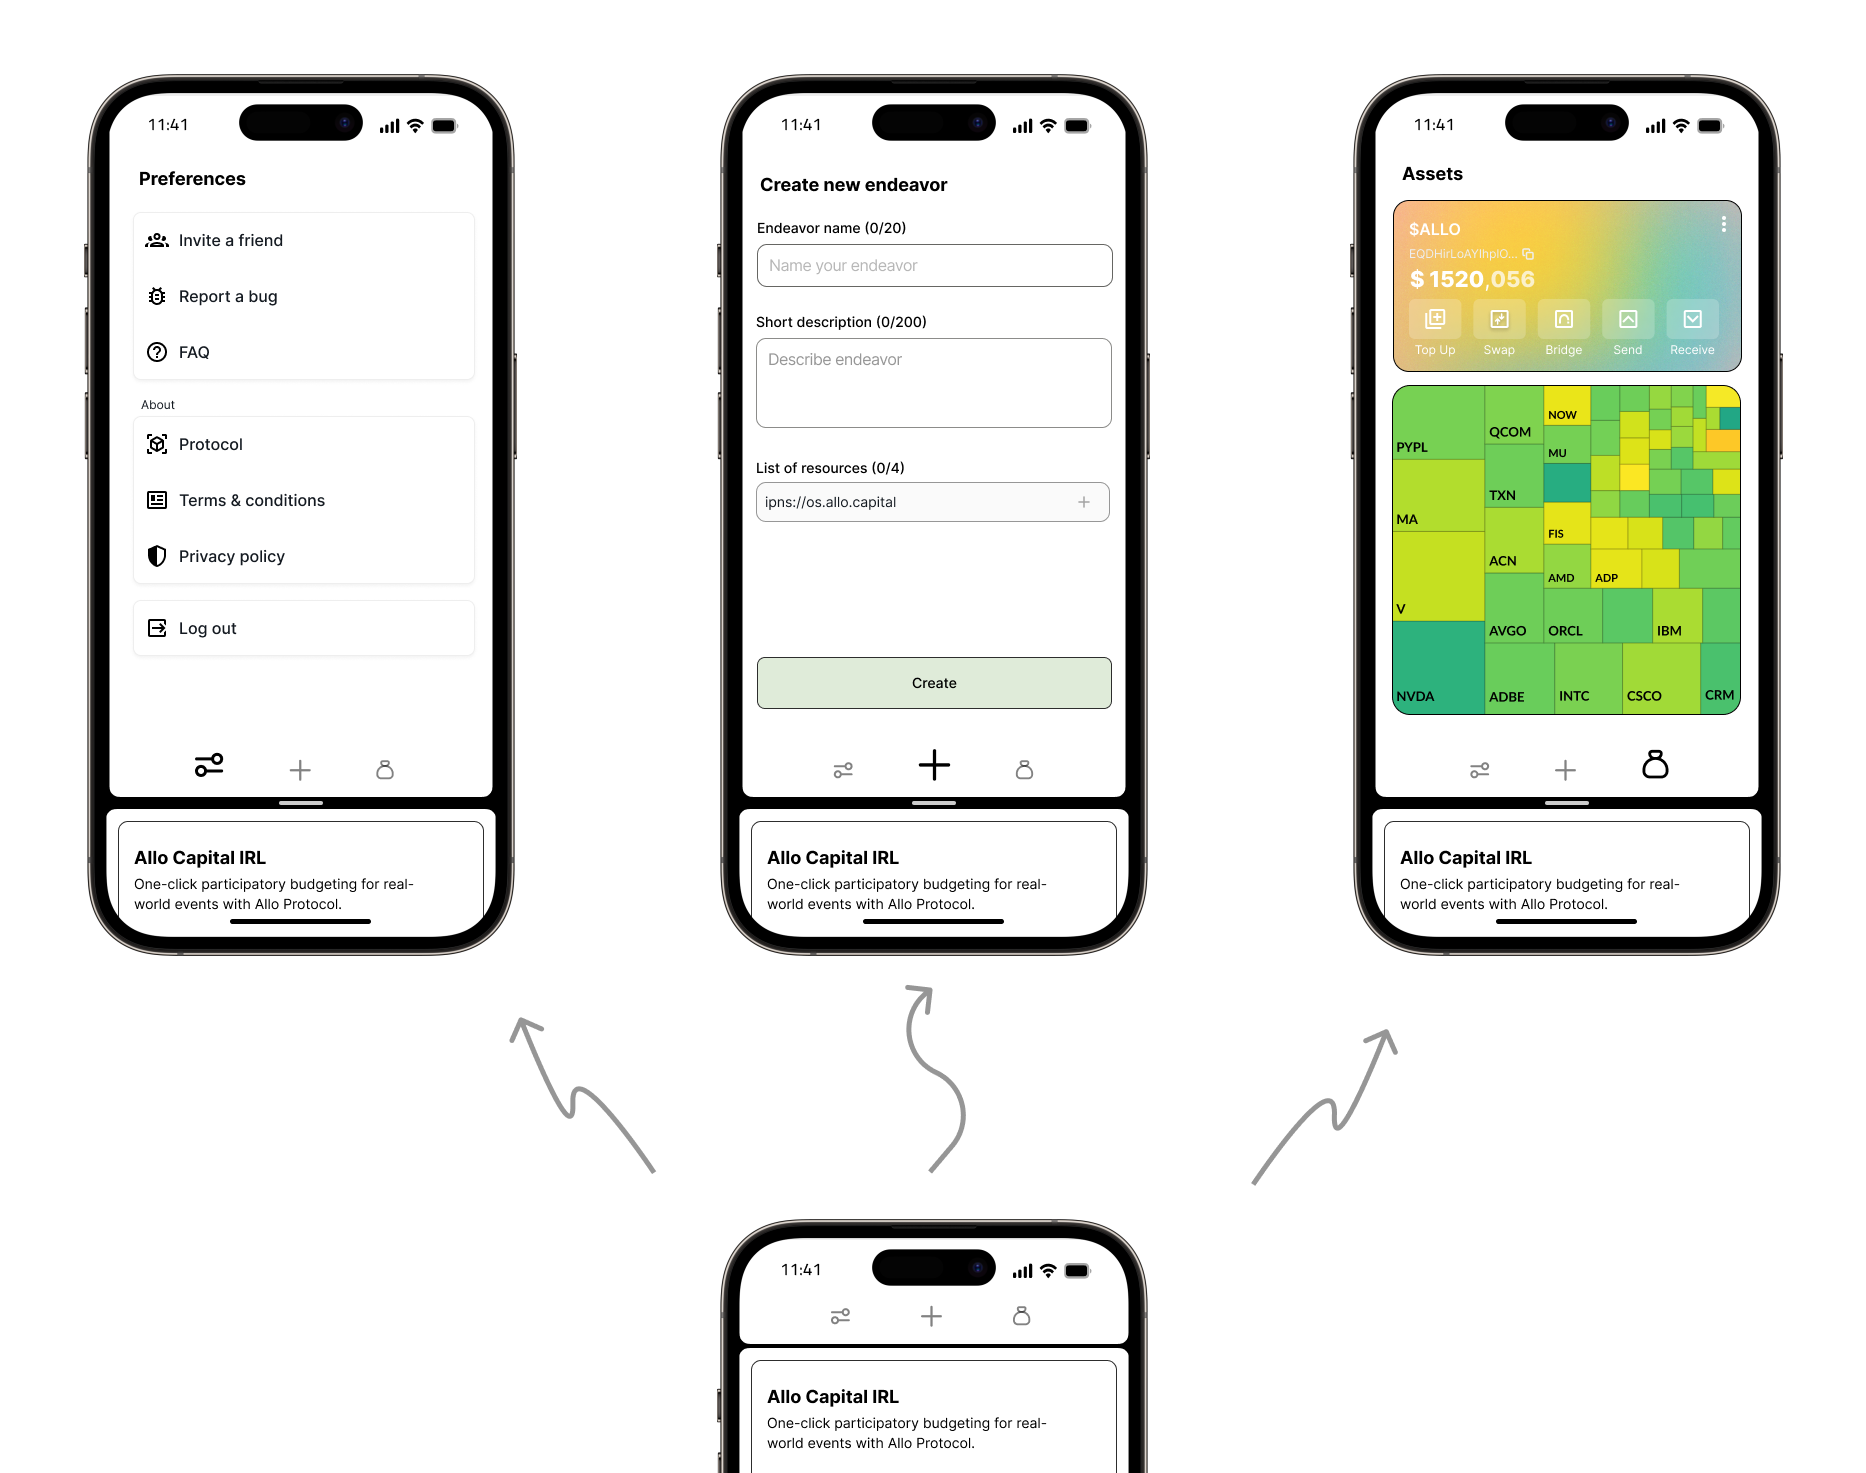
\includegraphics[width=0.5\textwidth]{./assets/app-navigation.png}
  \caption{Экран навигации между модулями приложения}
  \label{fig:app-navigation}
\end{figure}

% #### 4.5.2
\mysubsection{Экран управления активами и финансами}

Экран управления активами предоставляет пользователю сведения о его финансовых ресурсах в приложении. Здесь отображаются все доступные активы (например, внутренние токены или валюты, связанные с платформой).

Интерфейс организован в виде списка кошельков или счетов: каждая строка представляет отдельный актив с указанием его названия или тикера, идентификатора (например, часть адреса кошелька) и текущего баланса. В прототипе присутствует актив с кодом \$ALLO — рядом с ним показан уникальный идентификатор (адрес счёта или номер кошелька) и баланс, выраженный числом (например, 1,520,056).

Для каждого актива предусмотрены отдельные управляющие элементы: кнопки действий для управления средствами, такие как «Top Up» (пополнить), «Swap» (обменять), «Bridge» (перевести между сетями), «Send» (отправить) и «Receive» (получить). Ниже основного актива также отображается тепловая карта инвестиций по различным проектам, что позволяет пользователю визуально оценить распределение своих активов.

Типичный сценарий использования: пользователь переходит в этот раздел, чтобы проверить достаточен ли у него баланс для участия в той или иной инициативе, либо чтобы просмотреть результаты предыдущих взаимодействий.

% #### 4.5.3
\mysubsection{Экран создания новой инициативы}

Экран создания нового видео позволяет пользователю добавить свой собственный проект или предложение в систему. Это форма ввода данных, где последовательно представлены поля, необходимые для описания инициативы.

На экране отображается заголовок формы «Create» (Создать новую инициативу) для ясности. Далее следуют поля ввода: первое поле – название инициативы, ограниченное определённым количеством символов (в прототипе указано ограничение 0/20 символов, что означает максимальную длину имени 20 символов). Следующее поле – краткое описание инициативы (с ограничением 0/200 символов).

Затем присутствует блок для добавления связанных ресурсов или ссылок. В прототипе есть раздел «List of resources (0/4)», куда пользователь может добавить до четырёх ссылок на внешние ресурсы, связанные с инициативой. Один из примеров такого ресурса показан как ссылка на распределенное хранилище или страницу проекта.

После заполнения необходимых полей активируется кнопка «Create» (Создать), расположенная в нижней части формы. Нажатие этой кнопки сохраняет новую инициативу. Приложение при этом выполняет валидацию введённых данных и создает запись инициативы в системе.

% #### 4.5.4
\mysubsection{Экран настроек пользователя}

Экран настроек пользователя содержит опции для персонализации и обслуживания аккаунта. Этот раздел включает различные пункты, сгруппированные по тематике. В прототипе часть этих пунктов уже видна в меню навигации: например, «Preferences» (общие настройки), «Invite a friend» (приглашение новых пользователей), «Report a bug» (сообщение об ошибке разработчикам), «FAQ» (ответы на частые вопросы), и другие.

На экране настроек эти пункты представлены списком кнопок или ссылок. Нажатие на каждый из них приводит к соответствующему действию или открывает дополнительную информацию. Например, выбор «Preferences» открывает подэкран с настройками (переключателями и опциями, такими как уведомления, язык интерфейса). Выбор «Invite a friend» вызывает окно шаринга или копирует реферальную ссылку.

Экран настроек также отвечает за связь пользователя с системой в целом. Здесь расположен пункт «Log out» (Выход), с помощью которого пользователь может выйти из своего аккаунта или отключить текущую сессию.

С точки зрения сценариев, пользователь обращается к экрану настроек по необходимости: изменить что-то в профиле, узнать информацию о приложении, связаться с поддержкой или выйти из системы. Пример экрана настроек можно увидеть на рисунке.

Все представленные экраны в совокупности формируют комплексное пользовательское взаимодействие с платформой, обеспечивая доступ ко всему функционалу системы через интуитивно понятный мобильный интерфейс.

% ## 4.6
\mysection{Разработка клиентской части}

Мобильное приложение реализовано с использованием React Native и фреймворка Expo. Это позволило обеспечить мультиплатформенность и запуск приложения на iOS, Android, Web и Telegram Mini Apps без необходимости поддержки нескольких кодовых баз. React Native позволил повторно использовать UI-компоненты и бизнес-логику между платформами.

Архитектура приложения реализована по принципам Feature-Sliced Design (FSD), что обеспечивает модульность, предсказуемость структуры и лёгкость масштабирования. В соответствии с FSD, код организован в слои: app, pages, widgets, features, entities, shared. Каждый слой содержит тематические слайсы, разделённые на сегменты (ui, model, api, lib).

Для синхронизации клиентского состояния с сервером используется библиотека TanStack Query (ранее React Query). Она обеспечивает декларативное взаимодействие с API, кэширование запросов, автоматическое обновление данных и обработку ошибок. TanStack Query позволяет унифицировать доступ к данным и упрощает поддержку бизнес-логики, особенно в условиях высокой частоты обновления данных.

Для подключения к криптокошелькам в мобильной версии используется WalletConnect. Это открытый протокол, позволяющий подключать децентрализованные приложения к мобильным кошелькам с помощью QR-кодов или deep link-ссылок. Реализация WalletConnect обеспечивает механизм авторизации и безопасное взаимодействие с Web3-сервисами, отправку транзакций и подписание сообщений в пользовательском интерфейсе без прямого доступа к приватным ключам.

При реализации интерфейса особое внимание уделялось мобильной адаптивности и совместимости с Telegram Mini Apps. Использовались компоненты react-native-web и react-native-router, а для WebView-интеграции применялись средства Telegram WebApp SDK.

% #### 4.6.?
\mysubsection{Telegram Mini Apps}

Интеграция с Telegram реализована в двух форматах: Telegram-бот (asyncio): используется библиотека python-telegram-bot, которая предоставляет асинхронный интерфейс к Telegram Bot API. Бот обрабатывает команды администраторов (например, одобрение инициатив, блокировка пользователей), а также может принимать сообщения и отзывы от пользователей. Благодаря асинхронной модели бот способен масштабироваться и обрабатывать множество параллельных запросов, сохраняя отзывчивость. Бот работает через вебхуки или долгий опрос (polling), гарантируя своевременную реакцию на события (например, уведомление о завершении голосования).

Telegram Mini Apps это внутренняя веб-платформа Telegram, позволяющая запускать полнофункциональные веб-приложения (HTML/JS) внутри чата. Mini Apps используются для показа отдельного интерфейса (например, каталог инициатив или вкладка инвестирования) без необходимости переключаться в внешнее приложение. Это обеспечивает более «нативный» пользовательский опыт: Mini Apps «простой, гибкий, выглядит как родное веб-приложение, повышает удобство взаимодействия». С помощью Mini Apps пользователи могут, например, просматривать описание инициатив и совершать действия (голосовать, инвестировать) прямо из чата Telegram, получая полноценный UI, интегрированный в мессенджер.


% ## 4.7
\mysection{Вывод по четвертой главе}

В данной главе была описана реализация децентрализованного инвестиционного приложения в соответствии с архитектурной моделью, рассмотренной ранее. Мы рассмотрели бизнес-процессы (создание инициатив, коллективная оценка, распределение инвестиций и управление активами) и проиллюстрировали, как они поддерживаются выбранными технологиями. Архитектура системы комбинирует фронтенд на React/Expo с надёжной серверной частью на Python и реляционной БД PostgreSQL, дополняя её распределённым хранением данных через IPFS. Непрерывная интеграция и развертывание осуществляются с помощью GitHub Actions, что позволяет оперативно поставлять новые версии приложения. Клиентская часть обеспечивает удобные экраны (главный дашборд, создание инициатив, управление активами и др.), а интеграция с Telegram (бот и Mini Apps) открывает дополнительные каналы взаимодействия с пользователями. Таким образом, реализованный прототип приложения сочетает современные инструменты разработки с концепциями блокчейн-проектов и коллективного инвестирования, создавая основу для дальнейшего развития и внедрения в реальную экосистему.

% ###################################################
% ## Глава 5
% ###################################################

\mychapter{ПЕРСПЕКТИВЫ РАЗВИТИЯ}

\mysection{Масштабирование инвестиционной платформы}

Монетизация системы может происходить за счёт стейкинга пула ликвидности, а управление механизмом в перспективе может быть реализовано посредством community notes. В долгосрочной перспективе возможен выпуск стейблкоинов, обеспеченных пулами ликвидности и привязанных к стабильным активам, что значительно расширит функционал и доступность системы для пользователей и инвесторов.

Дальнейшее развитие платформы инвестирования организовано в виде последовательного поэтапного процесса, каждый этап которого имеет чётко определённые цели, задачи и показатели успеха. На первой фазе создаётся минимально жизнеспособный продукт, направленный на проверку ключевых концепций, привлечение ограниченной группы ранних пользователей, сбор первичной обратной связи и валидацию основных гипотез. В этот период реализуются базовые механизмы квадратичного финансирования, протоколы защиты интеллектуальной собственности и первичные пользовательские интерфейсы, что позволяет провести серию тестовых раундов финансирования и определить направления дальнейшего развития. Вторая фаза предусматривает запуск полнофункциональной версии платформы в основной сети, расширение аудитории посредством целевого маркетинга, оптимизацию операционных процессов и формирование сообщества, при этом реализуются более продвинутые версии ключевых механизмов, что позволяет обеспечить выполнение запланированных финансовых и эксплуатационных показателей. Третья фаза направлена на масштабирование функциональности и интеграцию с существующими экосистемами венчурного финансирования, что включает международную экспансию, адаптацию экономических механизмов на основе эмпирических данных и глубокую интеграцию с традиционными инвестиционными платформами, что приводит к значительному росту числа активных пользователей и объёмов привлечённого капитала. Четвёртая фаза предусматривает переход к полностью децентрализованной модели управления, создание открытой экосистемы для сторонних разработчиков, достижение самодостаточности экономической модели и становление платформы в качестве отраслевого стандарта для инвестирования в ранних стадиях инновационных проектов.

Стратегия масштабирования технологической инфраструктуры базируется на поэтапном увеличении вычислительных мощностей, расширении блокчейн-инфраструктуры, оптимизации систем хранения данных и сетевых решений. При этом особое внимание уделяется постепенному увеличению резервных мощностей, модульности отдельных компонентов и автоматическому выделению ресурсов в зависимости от текущих потребностей системы. В начальной фазе используется развертывание на Ethereum Layer 2 для баланса между безопасностью и транзакционными издержками, с последующим внедрением мультичейн-архитектуры и специализированных решений для оптимизации хранения данных и вычислений. Стратегия выхода на рынок строится на последовательном подходе, начиная с фокусирования на узких сегментах аудитории, таких как технологические стартапы и эксперты в области блокчейна, с последующим расширением до традиционных инвесторов и, наконец, до массового рынка. Привлечение пользователей осуществляется посредством специализированных демонстраций, программ раннего доступа, образовательных инициатив и масштабных маркетинговых кампаний, что позволяет постепенно формировать устойчивое и активное сообщество вокруг платформы. Эффективность данной стратегии оценивается с помощью ключевых метрик, таких как стоимость привлечения пользователя, коэффициент удержания, уровень вовлечённости и органический рост за счёт рекомендаций, что позволяет оперативно корректировать маркетинговые и технические решения.

\mysection{Обобщение результатов}

Стоит отметить, что при каждый агент может реализовываться аналогичная структура, образуя рекурсивно вложенную среду: на уровне мета-игры «правила игры» сами настраиваются (через AI-стирающую компоненту), а на нижних уровнях ведётся локальная оптимизация под заданные стимулы.


\mysection{Практическое применение}

Рассмотрим на примере контеста на Pond

Современные языковые модели (LLM) открывают новые возможности для оценки и фильтрации стартап-идей на ранних стадиях, особенно в условиях информационной асимметрии, когда полнота и точность данных ограничены. Аналогично роли бизнес-ангелов, описанной в работе \cite{lange2024angels}, LLM-системы могут выполнять функцию предварительной интеллектуальной фильтрации, позволяя автоматизировать процессы отбора, анализа и сопровождения инновационных проектов.

Контест на pond является подобной средой со скрытым механизмом оценки
Можем выбрать архитектуру или метрики для LLM модели

Примерами таких соревнований являются:

Экспериментальные соревнования, проведённые в рамках проектов \cite{cryptopond2025gg23} и \cite{cryptopond2025quantifying}, демонстрируют использование представленного метода, основанных на частично заданных эталонных ответах и агрегировании предсказаний участников. Центральной задачей этих контестов выступает распределение некоторой количественной величины (например, вклада участников в проект или релевантности объектов) по широкому множеству примеров, где прямое ручное аннотирование всего массива данных непрактично. Предлагаемый метод позволяет обойти это ограничение за счёт выборочного аннотирования небольшой подвыборки с последующим обучением на ней механизма агрегации.

На основе за \cite{lange2024angels}

\begin{figure}[h]
  \centering
  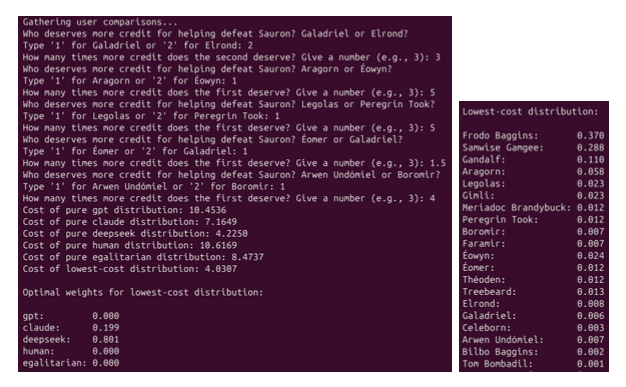
\includegraphics[width=0.5\textwidth]{./assets/llmcontest.png}
  \caption{Сравнение предел централизации и придела децентрализации}
  \label{fig:llmcontest}
\end{figure}

Процедура состоит из следующих этапов:

\begin{enumerate}
  \item Генерация оценок полного множества:
        Участникам (в том числе LLM-моделям или их гибридным конфигурациям) предлагается самостоятельно сформировать полный список численных оценок по всем экземплярам заданного множества. Например, участник должен оценить степень вклада каждого из $n$ агентов в некоторый проект. Модели не ограничиваются по способу получения ответа: допустимы как прямые алгоритмические предсказания, так и использование внешних источников, цепочек рассуждений, или даже краудсорсинг третьих агентов.

  \item Создание эталона (ground truth subset):
        Независимая экспертная комиссия (жюри) предоставляет «эталон» — небольшой поднабор ручных или полуавтоматических оценок, охватывающий малую часть исходного множества (например, 100 из 10 000 позиций). Эти оценки считаются высококачественными и выступают основой для проверки точности предсказаний.

  \item Определение наилучшего приближения:
        После получения всех поданных списков проводится численная процедура сопоставления: каждая предсказанная последовательность сравнивается с эталоном, и выбирается такая линейная комбинация предсказаний, которая минимизирует среднеквадратичную ошибку по выборке эталонных значений. Пусть $x_1, \dots, x_k$ — это векторы оценок, поданные участниками, а $y_{\text{true}}$ — эталонные оценки. Задача сводится к нахождению коэффициентов $\alpha_1, \dots, \alpha_k$, таких что:
        \[
          \min_{\substack{\alpha_i \ge 0 \\ \sum_{i=1}^k \alpha_i = 1}}
          \Bigl\lVert \sum_{i=1}^k \alpha_i x_i - y_{\text{true}} \Bigr\rVert_2^2.
        \]

        Решение этой задачи определяет не только итоговую агрегацию, но и относительное вознаграждение (или доверие), которое получает каждый участник за своё предсказание.

  \item Формирование финального результата:
        Полученная комбинация $\hat{y} = \sum \alpha_i x_i$ принимается как финальный ответ системы — агрегированная оценка по всему множеству объектов, максимально согласующаяся с мнением жюри на ограниченной выборке. При этом точечные ответы, которые наиболее точно отражают локальные закономерности в эталоне, получают больший вес в линейной смеси, независимо от их абсолютной производительности по всему корпусу.
\end{enumerate}

\mysection{Вывод по пятой главе}

Соединение воедино открывает возможности для маштабирования
Разработка такой системы для блокчейн принесет приемущества и вероятно откроет не только экономические применения
(однако консенсус невозможен)

% ###################################################
% ## Заключение
% ###################################################

\newpage
\begin{center}
  \textbf{ЗАКЛЮЧЕНИЕ}
\end{center}
\addcontentsline{toc}{chapter}{ЗАКЛЮЧЕНИЕ}

В рамках данной дипломной работы была разработана и исследована платформа слепого инвестирования в ранние стадии стартапов, основанная на блокчейн-технологиях и искусственном интеллекте. Работа была направлена на решение структурных проблем существующей системы венчурного финансирования, включая информационную асимметрию, субъективность оценок и риски для интеллектуальной собственности.

Ключевые результаты, достигнутые в ходе работы:

1. Проведен комплексный анализ существующих механизмов инвестирования в ранние стадии, выявлены их преимущества и ограничения. Определены основные проблемы, препятствующие эффективному распределению капитала для инновационных проектов.

2. Изучены и адаптированы передовые концепции и механизмы, включая квадратичное финансирование, возрастающие кривые ограничения и механизм распределения ресурсов с балансом автоматизации и человеческого контроля. Разработаны модификации этих механизмов для специфического контекста инвестирования в ранние стадии.

3. Разработана архитектура платформы, обеспечивающая защиту интеллектуальной собственности, объективную оценку проектов и оптимальное распределение капитала. Архитектура включает модули для управления проектами, механизмы инвестирования, аналитические движки и системы защиты интеллектуальной собственности.

4. Обоснован выбор технологического стека, включающего блокчейн Ethereum с решениями Layer 2 для обеспечения масштабируемости, криптографические протоколы для защиты данных, фреймворки искусственного интеллекта для оценки проектов и современные технологии для разработки пользовательских интерфейсов.

5. Разработан прототип платформы с ключевыми механизмами, включая протоколы защиты интеллектуальной собственности, системы оценки проектов, механизмы квадратичного финансирования и возрастающие кривые ограничения.

6. Проведена комплексная оценка эффективности предложенной платформы, включающая технические, функциональные, пользовательские и экономические тесты. Предварительные результаты показывают потенциал для 28\% повышения эффективности распределения ресурсов по сравнению с традиционными механизмами.

7. Разработаны рекомендации по интеграции и масштабированию решения, включая дорожную карту развития, стратегию выхода на рынок и направления дальнейших исследований.

Практическая значимость разработанной платформы заключается в создании новой парадигмы инвестирования, которая имеет потенциал для преодоления структурных ограничений существующих механизмов и обеспечения более эффективного распределения ресурсов для инновационных проектов. Это может способствовать ускорению технологического развития, созданию новых рабочих мест и повышению глобальной конкурентоспособности экономики.

Проведенное исследование также выявило ряд направлений для дальнейшей работы, включая совершенствование криптоэкономических механизмов, развитие технологий защиты интеллектуальной собственности, улучшение методов оценки проектов, исследование социально-экономических эффектов и развитие регуляторных подходов.

В целом, результаты работы демонстрируют значительный потенциал интеграции блокчейн-технологий, искусственного интеллекта и инновационных экономических механизмов для трансформации системы венчурного инвестирования в направлении большей эффективности, справедливости и доступности. Разработанная платформа представляет собой не просто технологическое решение, но комплексный подход к переосмыслению процессов распределения ресурсов для инновационных проектов, что имеет стратегическое значение для развития экономики знаний и инноваций.

\renewcommand{\bibname}{\fontsize{14pt}{21pt}\selectfont СПИСОК ИСПОЛЬЗОВАННЫХ ИСТОЧНИКОВ}
\bibliographystyle{bibformat}
\bibliography{bibliography}

\end{document}